%% 
%% Copyright 2007-2020 Elsevier Ltd
%% 
%% This file is part of the 'Elsarticle Bundle'.
%% ---------------------------------------------
%% 
%% It may be distributed under the conditions of the LaTeX Project Public
%% License, either version 1.2 of this license or (at your option) any
%% later version.  The latest version of this license is in
%%    http://www.latex-project.org/lppl.txt
%% and version 1.2 or later is part of all distributions of LaTeX
%% version 1999/12/01 or later.
%% 
%% The list of all files belonging to the 'Elsarticle Bundle' is
%% given in the file `manifest.txt'.
%% 

%% Template article for Elsevier's document class `elsarticle'
%% with numbered style bibliographic references
%% SP 2008/03/01
%%
%% 
%%
%% $Id: elsarticle-template-num.tex 190 2020-11-23 11:12:32Z rishi $
%%
%%
\documentclass[preprint,12pt]{elsarticle}

%% Use the option review to obtain double line spacing
%% \documentclass[authoryear,preprint,review,12pt]{elsarticle}

%% Use the options 1p,twocolumn; 3p; 3p,twocolumn; 5p; or 5p,twocolumn
%% for a journal layout:
%% \documentclass[final,1p,times]{elsarticle}
%% \documentclass[final,1p,times,twocolumn]{elsarticle}
%% \documentclass[final,3p,times]{elsarticle}
%% \documentclass[final,3p,times,twocolumn]{elsarticle}
%% \documentclass[final,5p,times]{elsarticle}
%% \documentclass[final,5p,times,twocolumn]{elsarticle}

%% For including figures, graphicx.sty has been loaded in
%% elsarticle.cls. If you prefer to use the old commands
%% please give \usepackage{epsfig}

%% The amssymb package provides various useful mathematical symbols
\usepackage{amssymb}
%% The amsthm package provides extended theorem environments
%% \usepackage{amsthm}

%% The lineno packages adds line numbers. Start line numbering with
%% \begin{linenumbers}, end it with \end{linenumbers}. Or switch it on
%% for the whole article with \linenumbers.
%% \usepackage{lineno}

\usepackage{multirow}
\usepackage{hyperref}
\usepackage{graphics}
\usepackage{booktabs}
\usepackage{multirow}
\usepackage{caption}
\usepackage{amsmath}
\usepackage{siunitx}

\journal{Journal of Hydrology}

\begin{document}

\begin{frontmatter}

%% Title, authors and addresses

%% use the tnoteref command within \title for footnotes;
%% use the tnotetext command for theassociated footnote;
%% use the fnref command within \author or \address for footnotes;
%% use the fntext command for theassociated footnote;
%% use the corref command within \author for corresponding author footnotes;
%% use the cortext command for theassociated footnote;
%% use the ead command for the email address,
%% and the form \ead[url] for the home page:
%% \title{Title\tnoteref{label1}}
%% \tnotetext[label1]{}
%% \author{Name\corref{cor1}\fnref{label2}}
%% \ead{email address}
%% \ead[url]{home page}
%% \fntext[label2]{}
%% \cortext[cor1]{}
%% \affiliation{organization={},
%%             addressline={},
%%             city={},
%%             postcode={},
%%             state={},
%%             country={}}
%% \fntext[label3]{}

\title{Issuing flood warnings at a continental scale: the case of the European Flood Awareness System}

%% use optional labels to link authors explicitly to addresses:
%% \author[label1,label2]{}
%% \affiliation[label1]{organization={},
%%             addressline={},
%%             city={},
%%             postcode={},
%%             state={},
%%             country={}}
%%
%% \affiliation[label2]{organization={},
%%             addressline={},
%%             city={},
%%             postcode={},
%%             state={},
%%             country={}}

\author[inst1]{Jesús Casado-Rodríguez}
\author[inst1]{Peter Salamon}
\author[inst2]{Stefania Grimaldi}
\author[inst2]{Corentin Carton De Wiart}
\author[inst2]{Christel Prudhomme}
\author[inst2]{Calum Baugh}
\author[inst2]{Ervin Zsoter}
\author[inst3]{Ilias Pechlivanidis}
\author[inst3]{Nina Bosshard}
\author[inst4]{Michaela Mikulickova}

\affiliation[inst1]{organization={European Commission, Joint Research Centre, Directorate E - Space, Security and Migration},%Department and Organization
            addressline={Via Enrico Fermi 2749}, 
            city={Ispra},
            postcode={21027}, 
            state={(VA)},
            country={Italy}}

\affiliation[inst2]{organization={European Centre for Medium Range Weather Forecasts},%Department and Organization
            addressline={Shinfield Park}, 
            city={Reading},
            postcode={WC2R 2LS}, 
            country={UK}}

\affiliation[inst3]{organization={Swedish Meteorological and Hydrological Institute},%Department and Organization
            city={Norrköping},
            country={Sweden}}

\affiliation[inst4]{organization={Slovak Hydrometeorological Institute},%Department and Organization
            city={Bratislava},
            country={Slovakia}}

\begin{abstract}
%% Text of abstract
The European Flood Awareness System (EFAS) of the Copernicus Emergency Management Service is an operational forecasting system whose aim is to raise awareness about floods in European transnational rivers. It produces probabilistic, medium-range discharge forecasts twice a day by running the open-source hydrological model LISFLOOD with four different meteorological forcing, two deterministic forecasts from the DWD (German Weather Service) and the ECMWF (European Centre for Medium Range Weather Forecasts), respectively, and two probabilistic forecasts from ECMWF and the Cosmo Consortium (COSMO-LEPS). Based on these forecasts, flood notifications are issued to the EFAS partners if a set of criteria is met: contributing area larger than 2000 km², lead time from 2 to 10 days, at least one deterministic model exceeds the discharge threshold (5-year return period), and at least one probabilistic model predicts 30\% exceedance probability of that discharge threshold for three or more consecutive forecasts. 
However, the operational EFAS is being regularly updated, so the configuration of EFAS has changed since the time these notification criteria were defined. For instance, the temporal resolution has increased from daily to 6-hourly, and the spatial resolution is planned to improve from 5km to approximately 1.5 km (1 arc-minute). 
This study aims at assessing the skill of the notification criteria above presented with the current system setup, and to derive a new set of criteria that optimizes the notification skill. We will focus on three research questions: (i) how can we combine the different models (deterministic and probabilistic) into a grand ensemble and what probability threshold optimizes skill? (ii) Is the persistence criterion (i.e. 3 consecutive forecasts need to provide persistent predictions of high flood risk) adding to the skill both at shorter and larger lead times? (iii) Can we reduce the contributing area threshold without compromising skill?
The study will make use of reanalysis, driven by meteorological observations, and forecast data at over 1200 points across Europe. By comparing the reanalysis data with the simulated discharge threshold, a total of 678 “observed” flood events have been identified in the years 2021 and 2022. We have tested 4 approaches in which to combine the 4 meteorological forcing and several combinations of the probability and persistence criteria. For each of the runs we computed binary classification skill metrics such as recall, precision and the f-beta score, and we have searched for the combination of criteria that maximizes this latter metric. We have also looked into how the skill of the system evolves with lead-time and catchment area.
The outcome of this study will be applied to the EFAS operational system, directly impacting the preparedness of the relevant authorities in future flood events.

\end{abstract}

%%Graphical abstract
%\begin{graphicalabstract}
% 
\includegraphics{grabs}
% \end{graphicalabstract}

%%Research highlights
% \begin{highlights}
% \item Research highlight 1
% \item Research highlight 2
% \end{highlights}

\begin{keyword}
%% keywords here, in the form: keyword \sep keyword
EFAS \sep flood warnings \sep floods early warning system \sep probabilistic forecasting
%% PACS codes here, in the form: \PACS code \sep code
\PACS 0000 \sep 1111
%% MSC codes here, in the form: \MSC code \sep code
%% or \MSC[2008] code \sep code (2000 is the default)
\MSC 0000 \sep 1111
\end{keyword}

\end{frontmatter}

%% \linenumbers

%% main text
\section{Introduction}
\label{sec:introduction}

The objective of this analysis is to assess the EFAS flood forecasting skill driven by the current formal notification criteria and to explore whether that skill can be improved by changing the current criteria for issuing formal notifications.

The research questions are the following:

\begin{enumerate}
    \item Total probability:
    \begin{itemize}
        \item How should the simulations based on the 4 meteorological forcing systems (of different characteristics and ensemble size) be combined in order to compute the total exceedance probability?
        \item What would be the optimal probability threshold that maximizes skill in notifying floods?
    \end{itemize}
    \item Persistence:
    \begin{itemize}
        \item Is forecast persistence a valuable criterion at both short (\textless 5 d) and long (\textgreater 5 d) lead times?
        \item Should the criteria be relaxed?
    \end{itemize}
    \item Can the existing upstream area threshold be reduced without reducing skill in issuing notifications?
\end{enumerate}

\section{Data}
\label{sec:data}

The data used in this analysis is taken from the operational setup of the European Flood Awareness  System (EFAS) in its version 4. EFAS generates a hydrological forecast twice a day (00 and 12 UTC) forced by the meteorological forecast of 4 different numerical weather prediction (NWP) models, whose characteristics are specified in Table \ref{tab:NWP_chars}. EFAS combines probabilistic models (COS and EUE) and deterministic models (DWD and EUD).

\begin{table}
    \centering
    \caption{Characteristics of the numerical weather prediction models used in EFAS4.}
    \footnotesize %\small
    \begin{tabular}{llllll} 
        \toprule
        Model & Provider & Acronym & \parbox{2cm}{Max.\\ lead time} & \parbox{2cm}{No.\\ ensembles} & \parbox{2cm}{Spatial \\ resolution} \\
        \midrule
        COSMO-LEPS & & COS & 5.5 days & 20 & $\sim$ 7 km \\
        ICON-EU/ICON & DWD & DWD & 7 days & 1 & $\sim$ 6.5-13 km \\
        HRES & ECMWF & EUD & 10 days & 1 & $\sim$ 9 km \\ 
        ENS & ECMWF & EUE & 10 days &  51 & $\sim$ 18 km \\ 
        \bottomrule
    \end{tabular}
    \label{tab:NWP_chars}
\end{table}

The study period spans from the release of EFAS4 in October 2020 until June 2023. For this period we will use the EFAS reforecasts as the discharge prediction and the EFAS reanalysis as a proxy of discharge observations. Using reanalysis as ground truth avoids the limitation of observational data, and removes model representation and calibration errors from the analysis. The previous data sets must be converted from a continuous variable (discharge) into binary events of exceedance or not exceedance over a threshold. Following the current EFAS setup, the flood threshold is the discharge associated with the 5 year return period, which was computed from the simulated discharge the EFAS4 long run (1991-2023)  by fitting a Gumbel distribution to the annual maxima.

Spatial resolution of EFAS!!

Unlike the original EFAS skill assessment \cite{Bartholmes2009}, the analysis will not focus on all the river cells in the model, which might cause a large autocorrelation problem, but only on what are called "fixed reported points" in EFAS jargon. From the almost 4000 fixed reporting points a selection was made based on two conditions: that the contributing area is larger than 500 km², and that the hydrological performance in terms of modified KGE (Kling-Gupta efficiency) \cite{Gupta2009, Knoben2019} is not lower than 0.50. In the end, 1979 fixed reporting points were included in the analysis, which account for a total of 1683 events (exceedances over the 5 year threshold) during the study period. As it will be explained in section \ref{sec:methods_OPT}, the optimization of the notification criteria will be done on the subset of 1239 reporting points whose contributing area is larger than 2000 km²; the total amount of events in this subset is 874.

Define what's a fixed reporting point!!



\section{Methods}
\label{sec:methods}

The analysis is organized in four steps, as seen in Figure \ref{fig:scheme}.

\begin{figure}
    \centering
    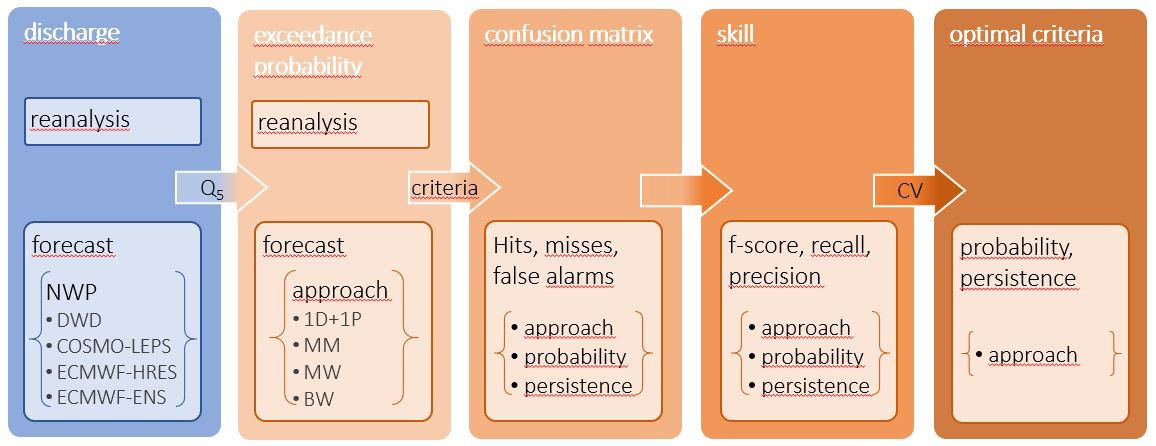
\includegraphics[width=0.9\textwidth]{figures/study_layout.JPG}
    \caption{Steps in the EFAS skill analysis and search for optimal notification criteria.}
    \label{fig:scheme}
\end{figure}

\subsection{Combination of NWP}
\label{sec:methods_COMB}

One of the main purposes of this study is to find an appropriate method to blend the deterministic and probabilistic forecasts. At this stage, we have converted the discharge forecasts into time series of exceedance or non exceedance over the 5-year return period ($Q_5$). In the case of the deterministic models, the exceedance time series is binary (0 or 1). In the case of the probabilistic models, supposing equiprobability among the members of the ensemble, the time series are probabilities of exceedance (range from 0 to 1). We will test 3 different ways of computing the total exceedance probability, and compare it with the current approach in EFAS, which does not use a total probability.

In the current EFAS procedure, a notification is issued if at least one deterministic and one probabilistic NWP predict the event. From now on we will refer to this approach as \textit{1 deterministic + 1 probabilistic} (1D+1P). Since every model is checked independently, this procedure does not compute a total probability matrix. The most simple approach to compute total probability is the \textit{model mean} (MM); the total exceedance probability is a simple mean over the four models, i.e., all models get an equal weight. In other words, the single member of the deterministic models are attributed a lot more importance than any of members of the probabilistic models. A different approach would be attributing the same weight to each member,  no matter if it belongs to a deterministic of a probabilistic model. We will term this approach as \textit{member weighted} (MW). In this approach each NWP gets a weight relative to the amount of members it contains, i.e., the probabilistic models prevail over the deterministic. None of the previous approaches take into account the performance of the NWP. To overcome this limitation, in the \textit{Brier weighted} approach (BW) the total exceedance probability each model gets a weight relative to its probabilistic skill. As a metric we have chosen the Brier score \cite{Brier1950}, a probabilistic error metric that ranges from 0 to infinite, with 0 being the optimal value. 

\begin{equation}
    \label{eq:BS}
    \text{BS} = \frac{1}{n}\sum_{i=1}^{n} \left( P_{obs} - P_{pred} \right)^2
\end{equation}

where $BS$  is the Brier score of a single reporting point, $n$  is the number of time steps, $P_{obs}$ is the observed probability of exceedance, and $P_{pred}$  is the predicted probability of exceedance. The conversion of the Brier score into weights proved to be of vital importance for the performance of this approach. The conversion function requires two things: it should invert the values from a metric whose optimal value is 0 to a weight whose optimal value is 1; it should be exponential to enhance the differences among NWP, given the low values of BS obtained, as it could be expected in a rare event where in the vast majority of the time steps both observed an predicted probabilities are 0. Inverse distance weighing (eq. \ref{eq:IDW}) fulfils both conditions. We tested values of the exponent $p$ from 1 to 9 and discovered that 7 was the optimal value.
    
\begin{equation}
    \label{eq:IDW}
    w = \frac{BS^{-p}}{\sum BS{-p}}
\end{equation}
Both the Brier scores and their associated weights are specific for a NWP and a lead time. Whereas the weights in the MM and MW approaches are stable in time, this approach assigns different weights to each model at every lead time.

\subsection{Contingency table}
\label{sec:methods_contingency}

The flood notification skill assessment is a binary classification task in which we compare two time series: the predicted and the observed events. In such classification  problems, the contingency table (Table \ref{tab:contingency_table}) summarizes the outcome of the model and its four terms are used to assess the skill (see section \ref{sec:methods_metrics}). Floods are rare events, which means that the classification task is highly imbalanced and the amount of true negatives will be orders of magnitude larger than any of the other terms. For that reason, the true negatives will be disregarded both in the computation of the contingency table and in the selection of the target skill metric.

\begin{table}
    \centering
    \caption{Contingency table in a binary classification.}
    \footnotesize
    \begin{tabular}{ccccc}
        \toprule
        & & \multicolumn{2}{c}{Observed} & \\
        \cmidrule{3-4}
        & & True & False & \\
        \midrule
        Forecasted & True & hit & false alarm & $E_{pred}$ \\
        & False & miss & true negative & \\
        &  & $E_{obs}$ & & \\
        \bottomrule
    \end{tabular}
    \label{tab:contingency_table}
\end{table}

The derivation of the binary time series of observed events is straight forward by application of the discharge threshold ($Q_5$) over the discharge reanalysis. The derivation of the binary time series of forecasted events requires the application of the notification criteria over the matrix of total probability of exceedance (or the independent matrices of exceedance probability for each NWP in the 1D+1P approach). 

Two are the notification criteria involved in this step. The probability threshold establishes the minimum value of the exceedance probability from which we consider that there is a high risk of flooding that must be notified to the EFAS partners. In the current procedure, the threshold is 30\% and it applies only to the probabilistic forecasts (approach 1D+1P). The persistence was a criteria introduced to remove false alarms caused by the erratic behaviour of some NWP \cite{Bartholmes2009}. The idea was to replicate the behaviour of a forecaster, who would wait to send the warning until consecutive forecasts predict the event. In the current procedure, notifications are sent if 3 consecutive forecasts exceed the probability threshold (from know on we will refer to this persistence as 3/3, three out of three). 

Figure \ref{fig:procedure} illustrates how these two notification criteria are applied on the matrix of predicted exceedance probability. For every time step, the gray outline identifies the lead times that comply with the criteria (the example shows the current EFAS criteria). The predicted events are the time steps for which at least one lead time complies with the criteria; notice that the matrix starts at lead time 2 days because that is the minimum lead time in the EFAS notifications. The terms of the contingency table result from the comparison of the predicted and observed events. We consider a hit any observed event in which at least one time step was correctly predicted. The number of misses or false alarms are directly computed by the difference between the observed or predicted events, respectively, and the hits.
\begin{figure}
    \centering
    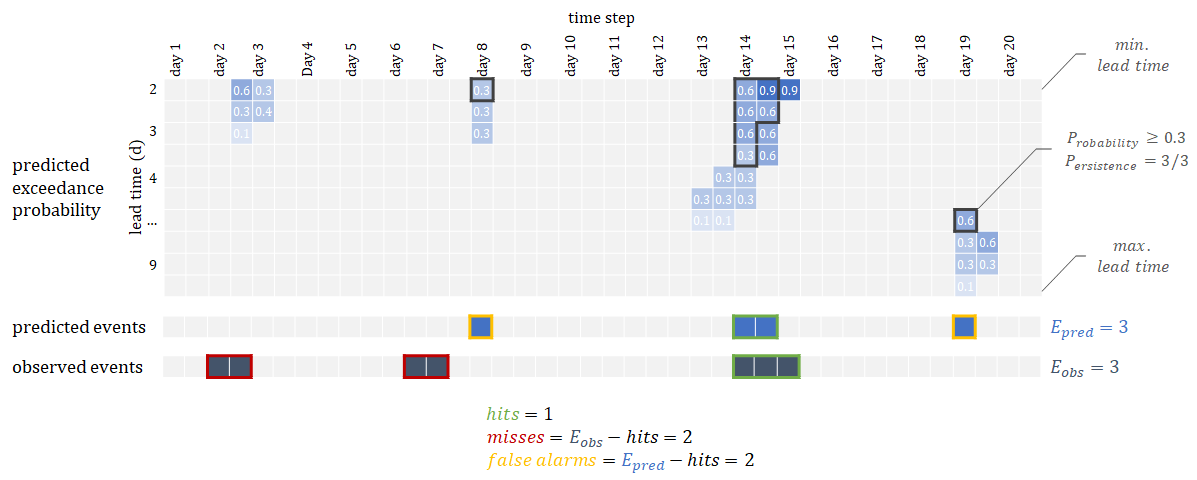
\includegraphics[width=1\textwidth]{figures/explanation_procedure.PNG}
    \caption{Illustration of the procedure applied to compute the values of the contingency table for the current notification criteria. On top, the matrix of probability of exceeding the discharge threshold. The probability and persistence criteria are applied on that matrix to derive a time series of predicted events. Hits, misses and false alarms are computed by comparing the time series of predicted and observed events.}
    \label{fig:procedure}
\end{figure}

The previous process is repeated for every reporting point and every combination of the two notification criteria. We have tested values of the probability threshold ranging from 5\% to 95\% and six persistence values: 1/1, 2/4, 2/3, 2/2, 3/4 and 3/3; where 1/1 means no persistence, 3/3 is the current criteria of three consecutive forecast predicting the event, and 2/4, for instance, is a persistence that requires 2 out of 4 consecutive forecasts predicting the event. The output of all this process are matrices of hits, misses and false alarms for each reporting depending on the probability threshold and persistence.

\subsection{Skill metrics}
\label{sec:methods_metrics}

The fact that the classification task we face is highly imbalanced is fundamental in the selection of the skill metric from the myriad of options. For instance, the odds ratio and the Hanssen-Kuipers score ($HK$) \cite{Hanssen1965} were discarded because both include the true negatives in their formulation, which is something we want to exclude in an imbalanced classification. Instead, we have chosen metrics that only use the hits, misses and false alarms. Instead, we have selected three skill metrics specific for imbalanced classification, i.e., that exclude the true negatives. 

Recall is the proportion of observed events that are correctly predicted (eq. \ref{eq:recall}); in some contexts it is also known as hit rate, probability of detection or sensitivity. Bartholmes \cite{Bartholmes2009} proved that recall is equal to HK for highly imbalanced classifications as it is the case of floods. Precision, a.k.a. positive predicted value or frequency of hits, is the proportion of the predicted events that are correct (eq. \ref{eq:precision}). There is a well known trade-off between recall  and precision. In the specific case of flood notifications, very strict criteria would cause very few notifications with high certainty, which means that they will be mostly correct (high precision), but we would miss a lot of events (poor recall). On the other hand, very relaxed criteria would cause a large amount of uncertain notifications, which means that we would not miss events (high recall) but we would issue many false alarms (poor precision). The $f_{\beta}$ score  is a metric that balances recall  and precision (eq. \ref{eq:fscore}). In its most common version ($\beta = 1$) it is the harmonic mean of recall and precision, granting equal importance to both metrics. However, higher importance can be given to precision ($\beta < 1$), therefore limiting the amount of false alarms, or to recall ($\beta > 1$), so that it limits the amount of misses. After suggestions from the EFAS dissemination centre, we chose $f_{0.8}$ as the target skill metric. This metric balances precision and recall giving a slightly higher value to the former. The idea behind is to limit the amount of false alarms, which would jeopardize the trust of the EFAS partners. All the previous variables range from 0 to 1, being 1 their optimal value.

As a last validation metric we will use the bias, i.e., the proportion between the predicted and observed events, which turns out to be the quotient between recall and precision (eq. \ref{eq:bias}). Its optimal value is 1 and it ranges from 0 to infinity. All the four metrics here presented can be plotted in Roebber diagrams \cite{Roebber2009}. We will modify the original Roebber diagrams and replace the critical success index by our target metric ($f_{0.8}$).
\begin{equation}
    \text{recall} = \frac{\text{hits}}{E_{obs}} = \frac{\text{hits}}{\text{hits} + \text{misses}}
    \label{eq:recall}
\end{equation}
\begin{equation}
    \text{precision} = \frac{\text{hits}}{E_{pred}} = \frac{\text{hits}}{\text{hits} + \text{false alarms}}
    \label{eq:precision}
\end{equation}
\begin{equation}
    f_{\beta} = \left( 1 + \beta \right)^2 \frac{\text{precision} \cdot \text{recall}}{\beta^2 \cdot \text{precision} + \text{recall}}
    \label{eq:fscore}
\end{equation}
\begin{equation}
    \text{bias} = \frac{E_{pred}}{E_{obs}} = \frac{\text{hits} + \text{false alarms}} {\text{hits} + \text{misses}} = \frac{\text{recall}}{\text{precision}}
    \label{eq:bias}
\end{equation}

\subsection{Optimal notification criteria}
\label{sec:methods_OPT}

The notification criteria involve 5 variables: catchment area, lead time, combination of NWP, probability threshold and persistence. We will analyse and optimize all these variables, but we will isolate them to understand what are the effects of each of them.

We have conducted two main experiments to explore the benefits of combining NWP. The first experiment analyses individually the NWP. The objective is to identify the strengths and weaknesses of each of the NWP, and learn how the other notification criteria affect differently the probabilistic and deterministic NWP. The second experiment compares the 4 combinations of NWP explained in section \ref{sec:methods_COMB}. The objective is to identify the most appropriate combination method and compare it against the most skillful NWP, to assess whether the combination of NWP adds value to the system or not. The setup of these two experiments is similar, apart from the difference in the input data, and is explained in the following paragraphs.

For most of the analyses we have kept only the reporting points that comply with the current minimum catchment area of (2000 km²). With these reporting points, we explored the evolution of skill with lead time, probability and persistence. In this exploration, the 20 lead time values (2 values per day for an horizon of 10 days) were grouped in two ways. We grouped them daily to analyze the evolution of skill with lead time. To explore the impacts of the probability threshold and persistence we defined 4 lead time ranges: a) shorter than 2 days, a range at which formal notifications cannot be issued, b) 2-5.5 days, when all NWP are available, c) 5.5-7 days, when 3 NWP are available as the maximum lead time of COS is exceeded, d) 7-10 days when only 2 NWP are available as the maximum lead time of DWD is exceeded.

After exploring, we optimized the probability threshold and the persistence criteria. That is, we searched for the combination of probability and persistence that produces the maximum $f_{0.8}$ at each of the 4 lead time ranges. The search was repeated for every individual NWP and every combination of the NWP. To conduct a robust selection of criteria, we applied a 10-fold cross validation; 20\% of the reporting points were left aside as a test set, and the remaining 80\% of points were subdivided in 10 folds. We computed the skill for every combination of 9 folds and then averaged over folds. The optimal notification criteria was extracted from this average-over-fold skill matrix. The selected criteria was evaluated on the test set to prevent overfitting. 

There remains a criterion that has not been explored yet, the minimum catchment area. We first explored the evolution of skill for values of the minimum catchment area ranging from 500 km² to 300,000 km², given the criteria optimized in the previous step. Then, we only fixed the persistence criterion to that obtained in the optimization, and we optimized the probability threshold according to catchment area. The objective of this experiment is to check if the skill of the system, specifically that of small catchments, significantly improves with a more complicated notification criteria in which the probability threshold varies with catchment area.

Shouldn't the criteria be optimized for 1000 km2 instead of 2000 km2, since that will be the new minimum catchment area????

\section{Results}
\label{sec:results}

\subsection{Analysis of "observed" events}
\label{sec:obs_events}

Figure \ref{fig:map_observed} shows the geographical distribution of the 1239 reporting points used in the optimization; colours represent the amount of "observed" flood events. There is a higher proportion of stations with events in Central Europe, British Isles and the Mediterranean catchments than in Eastern and North-Eastern Europe. During the study period there were major events in the Rhine, Meuse and Ebro, which can be spotted in the map. 61\% of the reporting points did not exceed the 5 year return period during the study period. This means that in this proportion of the sample we cannot predict neither hits nor misses; the only term of the contingency table that we can derive for these 61\% of points are false alarms, which means that the f-score  can be either nonexistent or 0. On top of that, the percentage of reporting points with only 1 "observed" event is 29\%; for these points the f-score can only be either 0 or 1. These two facts have an implication in the overall skill of the system, as we will see later on.

\begin{figure}
    \centering
    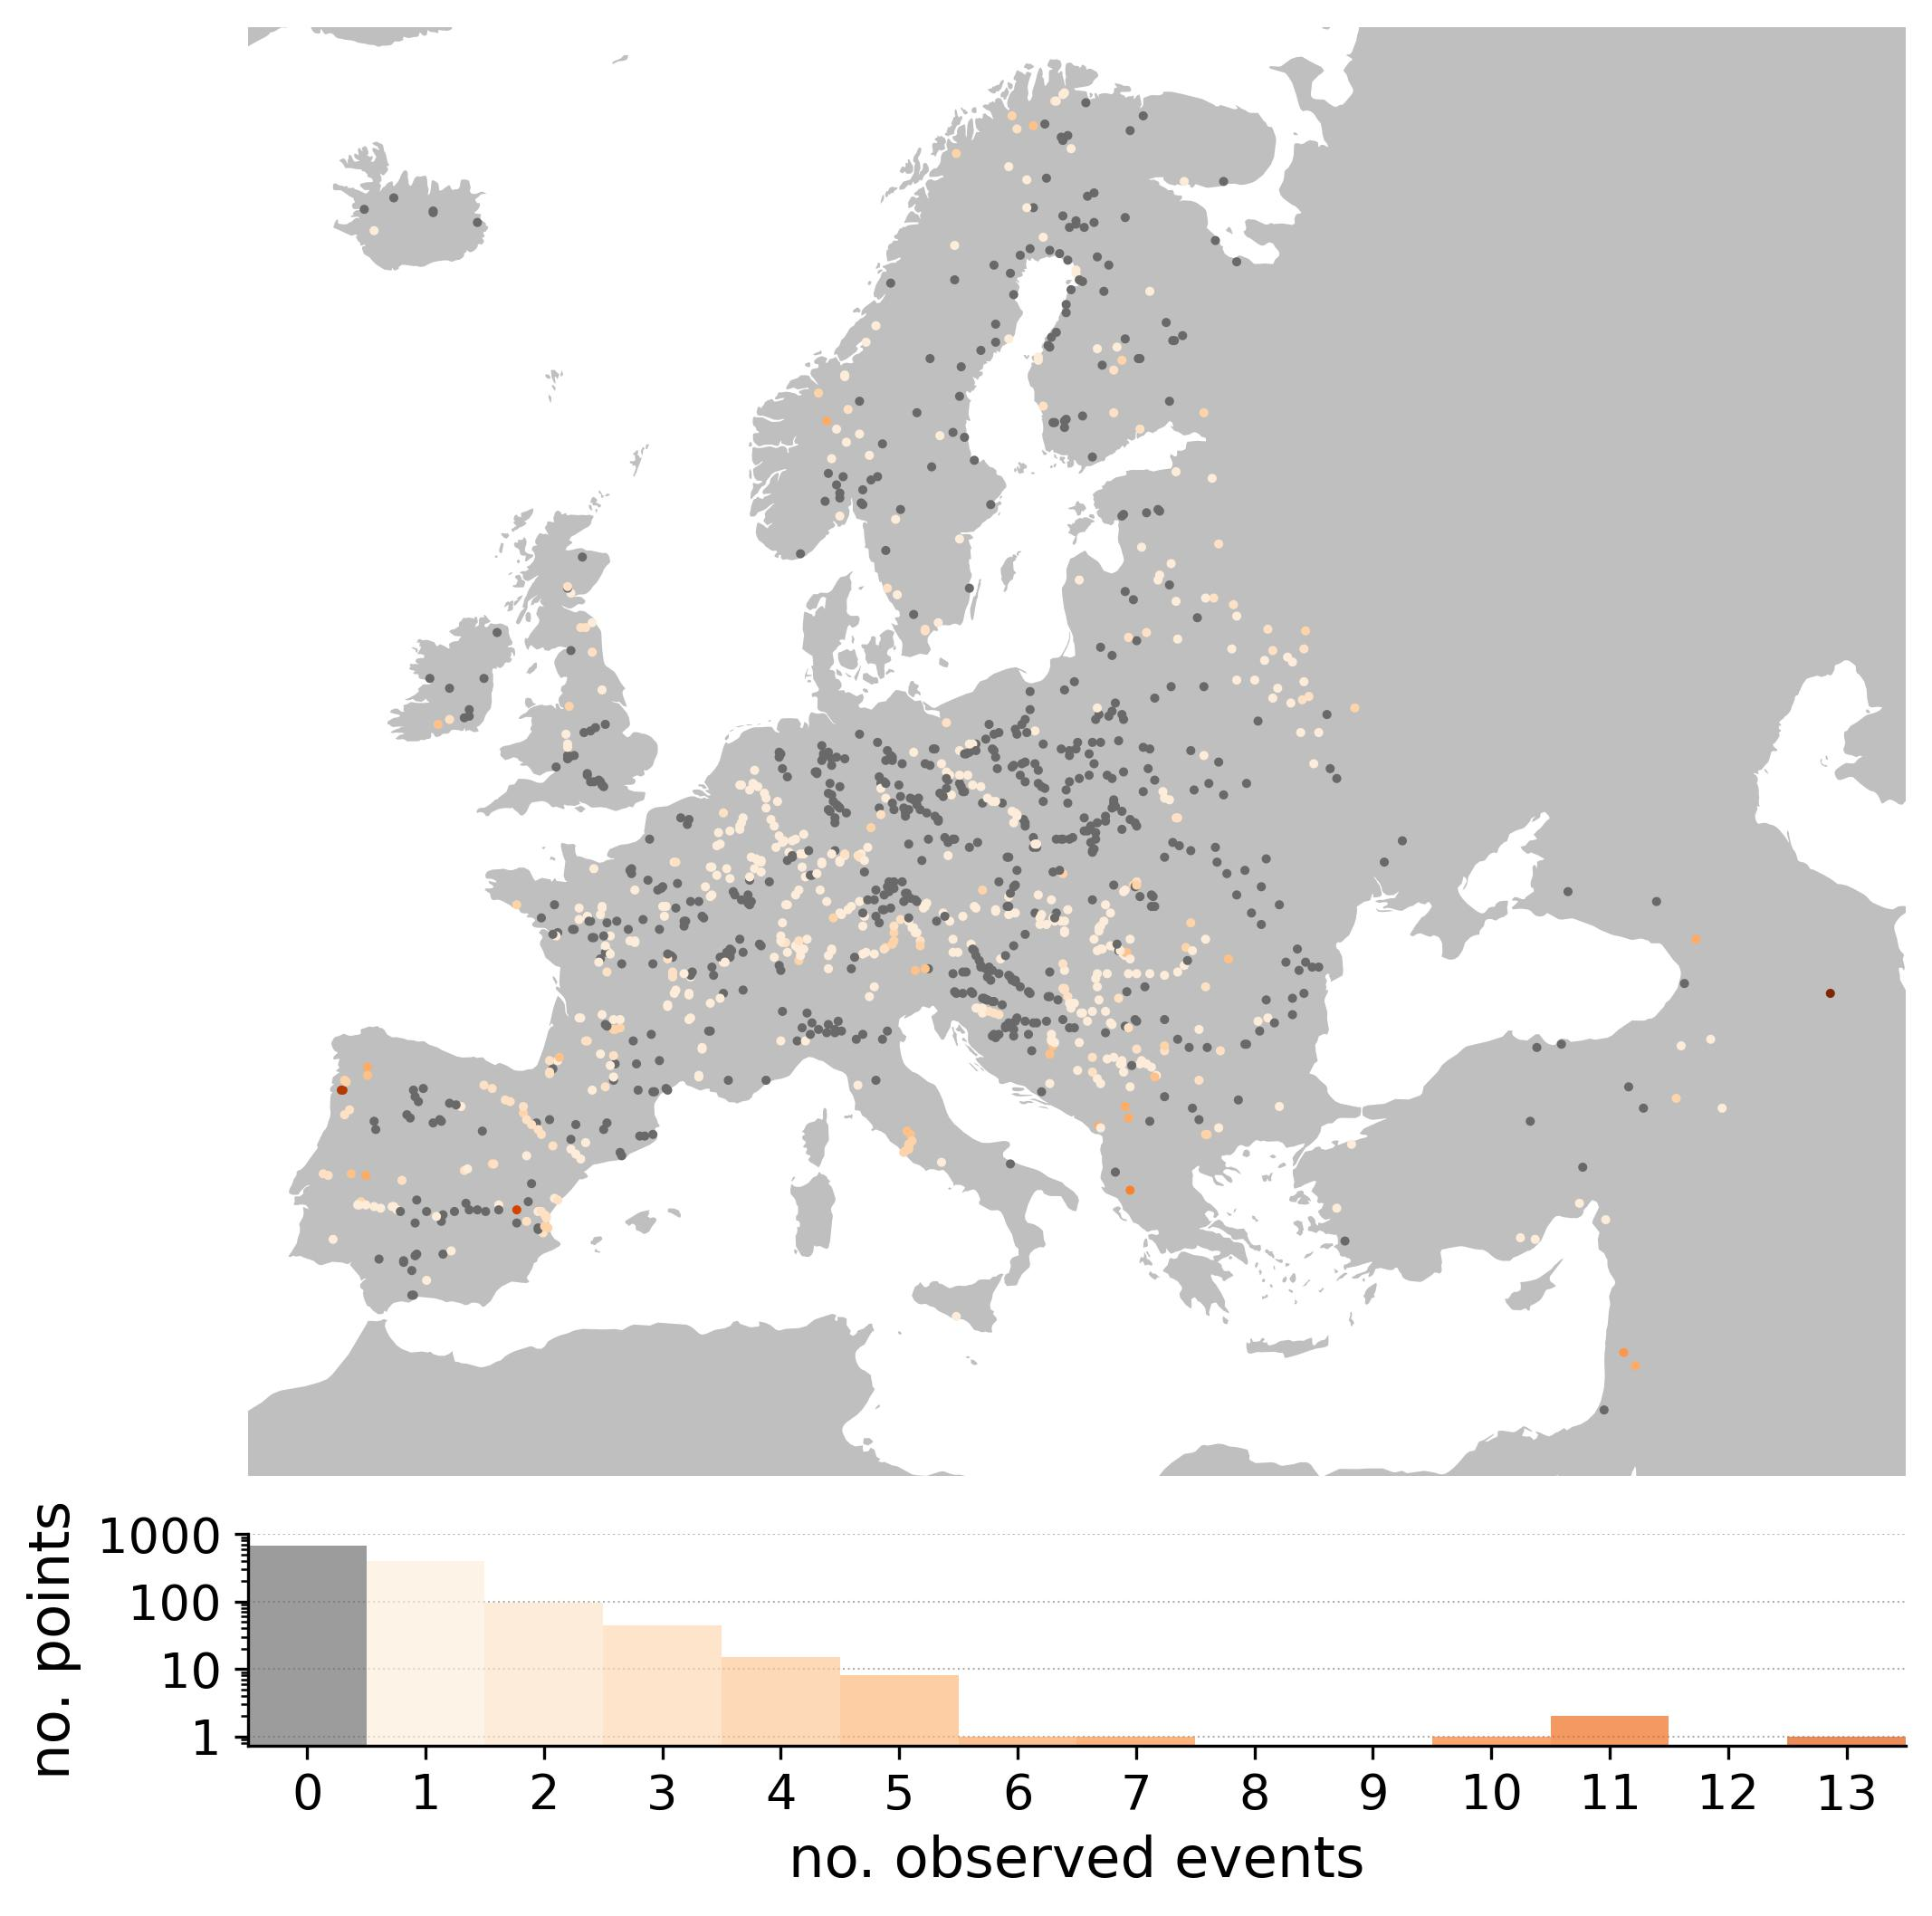
\includegraphics[width=0.5\linewidth]{figures/map_observed_events_2000km2_1239points.jpg}
    \caption{Geographical distribution of the fixed reporting points used for the criteria optimization and number of "observed" flood events during the study period.}
    \label{fig:map_observed}
\end{figure}

The distribution of the catchment size of the fixed reporting points is also uneven. Figure \ref{fig:observed_vs_area} represents both the number of fixed reporting points and the number of "observed" events over an increasing catchment area threshold. Note that the X axis is in logarithmic scale, and that the primary Y axis (reporting points) has a scale double than the secondary Y axis (events). Both the number of reporting points and the number of events decrease exponentially with catchment area. Since we will optimize the notification criteria for the current area limit of 2000 km², we discard 37\% of the reporting points and 48\% of the events.

\begin{figure}
    \centering
    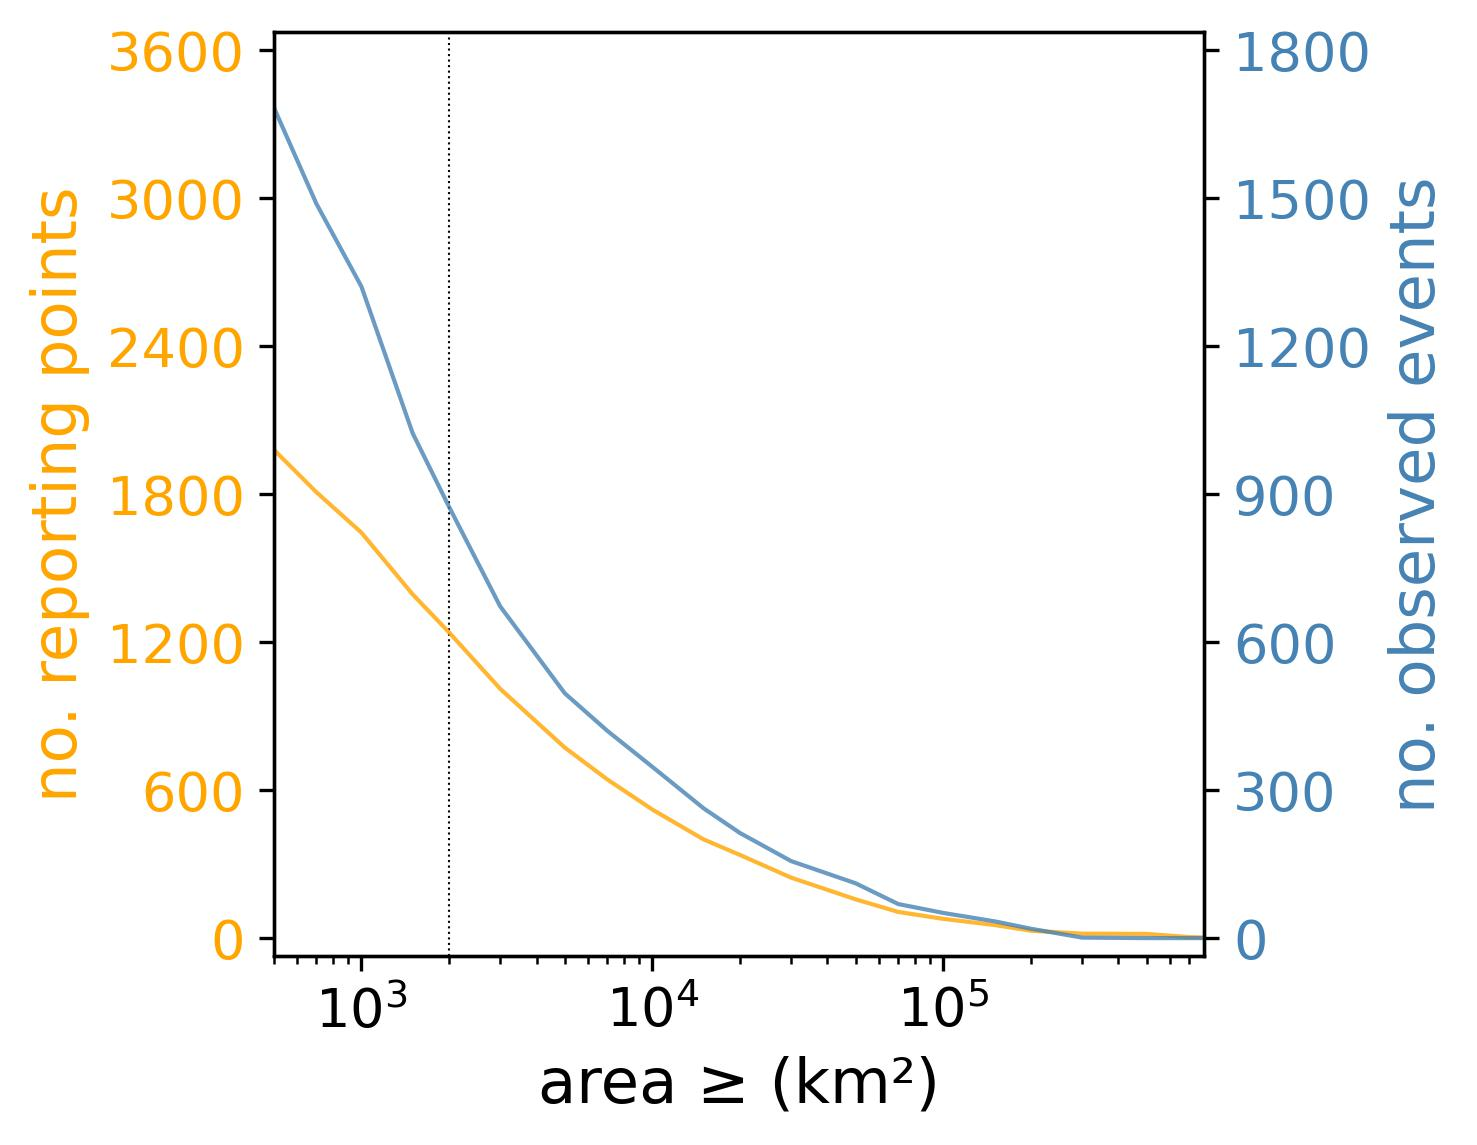
\includegraphics[width=0.5\textwidth]{figures/points_observedEvents_vs_area_2000km2_1239points.jpg}
    \caption{Number of reporting points (orange) and observed events (blue) by catchment area. The vertical, dotted line represents a catchment area of 2000 km², the current limit in the notifications.}
    \label{fig:observed_vs_area}
\end{figure}

We have also looked into the duration of the "observed" flood events (Figure \ref{fig:event_duration}), considering the duration of the event as the period of time in which discharge exceeds the 5-year return period. The majority of the events have a duration shorter than 2 days, both for the complete set of reporting points (78\% of the events) and the set that will be used in the optimization (72\%). Some events exceeded the discharge threshold for only one time step (6 h), which may represent events particularly difficult to predict; they account for 14\% and 11\% of the events in the complete and optimization sets, respectively. Even though the number of events is reduced to almost a half between the 500 km² and the 2000 km² thresholds (see Figure \ref{fig:observed_vs_area}), the distribution of the event duration is fairly similar. The figure limits the duration to 16 days for visualization reasons; nonetheless, there were 56 and 37 events longer that 16 days in the two sets of reporting points (approximately 3\% and 4\% of the events).

\begin{figure}
    \centering
    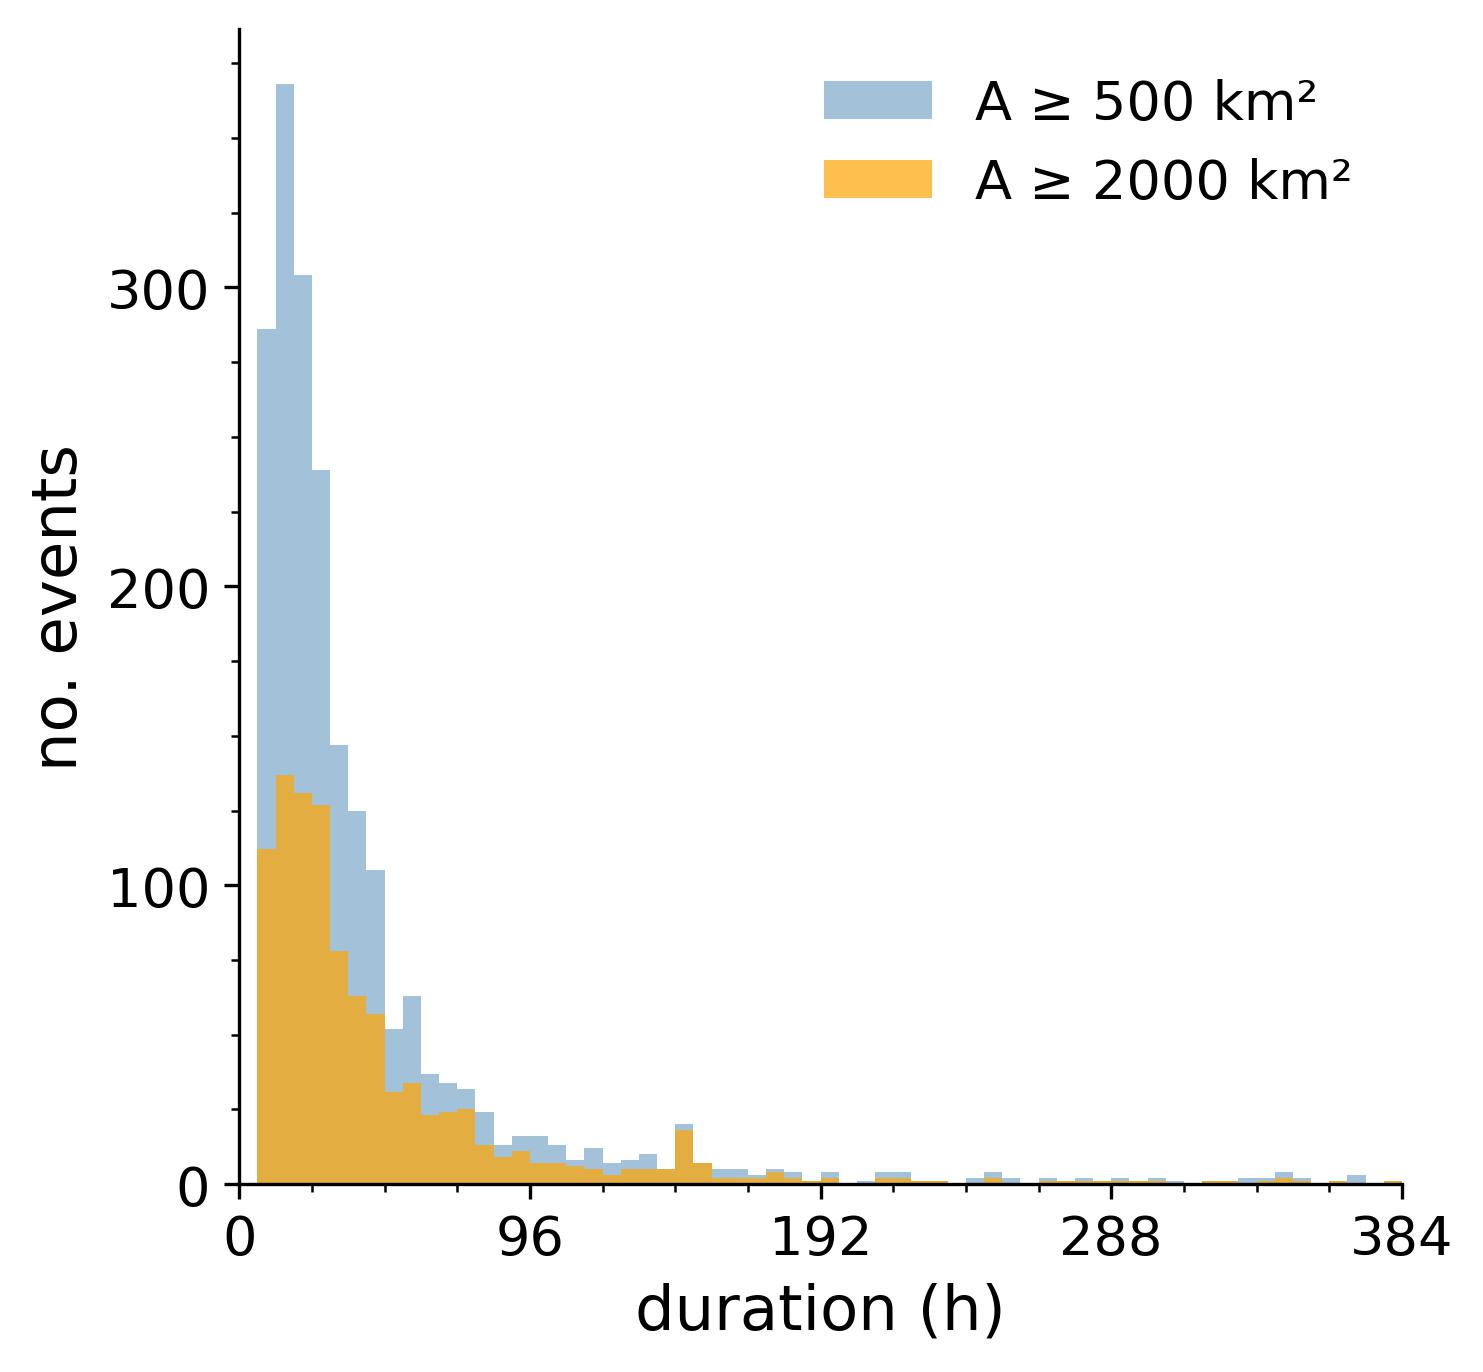
\includegraphics[width=0.5\textwidth]{figures/duration_distribution_2371points.jpg}
    \caption{Distribution of the duration of the "observed" flood events. Every bin corresponds to 6 h, i.e., the time step resolution. Blue represents all the reporting points included in the analysis, and orange the reporting points that will be used in the optimization of the notification criteria.}
    \label{fig:event_duration}
\end{figure}

\subsection{Individual NWP}
\label{sec:results_NWP}

Before studying how to combine the numerical weather prediction (NWP) models, we analysed the skill of each of the models individually. There are two objectives in this analysis. First, understand which models are more skillful in order to include this skill in the computation of total probability. Second, to compare the skill  of individual NWP models against the benchmark, the current notification criteria.

\subsubsection{Probabilistic skill}
\label{sec:NWP_prob_skill}

As a first approach to the NWP skill, we computed the Brier score for each NWP at daily lead times. The Brier score is an error metric whose values are errors not easy to interpret because the magnitude of the error depends on the variable at hand, which in the case of rare events like floods is very low. Instead, the Brier skill score (BSS) represents the relative skill of a model compared to a reference; models stronger than the reference get positive BSS, whereas models weaker than the reference get negative BSS. We selected as a reference a dummy model that never predicts an event ($P_{pred}=0$) \cite{Legg2004}.

\begin{figure}
    \centering
    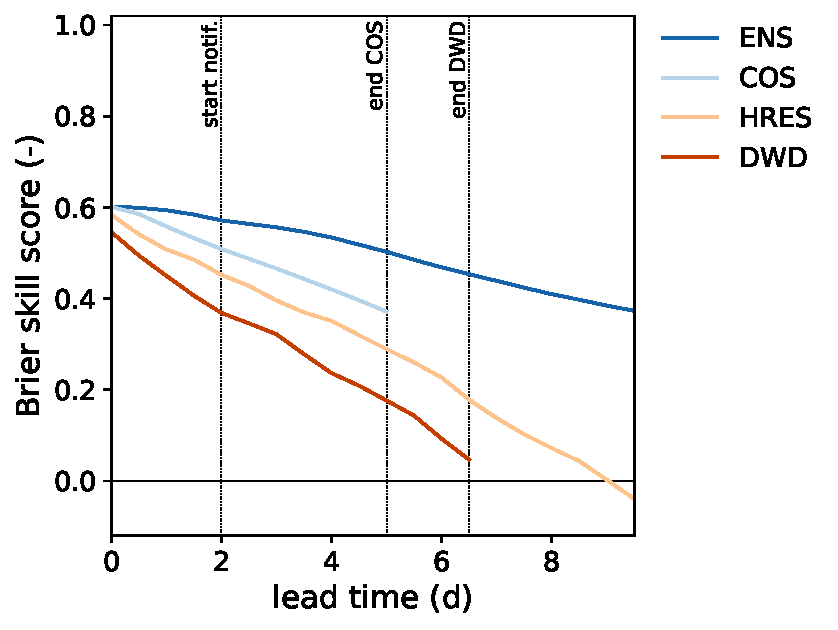
\includegraphics[width=0.5\textwidth]{figures/Brier_skill_score_5.pdf}
    \caption{Brier skill score of the four NWP used in EFAS at daily lead times. The reference ($BSS=0$) is a model that never predicts an event. Blue lines represent probabilistic models, and orange lines deterministic ones.}
    \label{fig:BSS}
\end{figure}

The plot above proves that probabilistic models are more skillful than deterministic ones. Only for very short lead times (0-1 days) the deterministic models show a skill close to the probabilistic models. This is important for EFAS notifications, since we do not send formal notifications with less than 2 days lead time (leftmost dotted line). As lead time increases, the skill of the predictions degrades; this degradation affects less EUE than the other models. The two deterministic models have poor skill at their forecast horizon; in the case of EUD at 10 days lead time the skill is worse than a model that never predicts a flood. Overall, the most skillful model is EUE and the less skillful is DWD. In section \ref{sec:results_COMB} the Brier scores will be converted into weighing factors for the computation of total probability (see Figure \ref{fig:weights}).

\subsubsection{Notification skill}
\label{sec:NWP_skill}

In this section we analysed how the NWP would have performed if notifications would be sent based uniquely in one of them. First, we want to have a general picture of how notification skill evolves according to the 3 dimensions here involved (lead time, probability threshold and persistence). Second, we will optimize the probability and persistence criteria for a fixed lead time.

Figure \ref{fig:NWP_skill_leadtime} exhibits the evolution of the notification skill with lead time and probability threshold for a scenario with no persistence. The black, solid line is the notification skill of the current notification criteria, as a benchmark to compare the skill of the individual NWP models. Every colour line represents a different probability threshold; orange lines represent thresholds below 50\% and blue lines over that value. For the two deterministic models (DWD, EUD) all lines overlap, since the probability threshold does not affect a deterministic forecast.

\begin{figure}
    \centering
    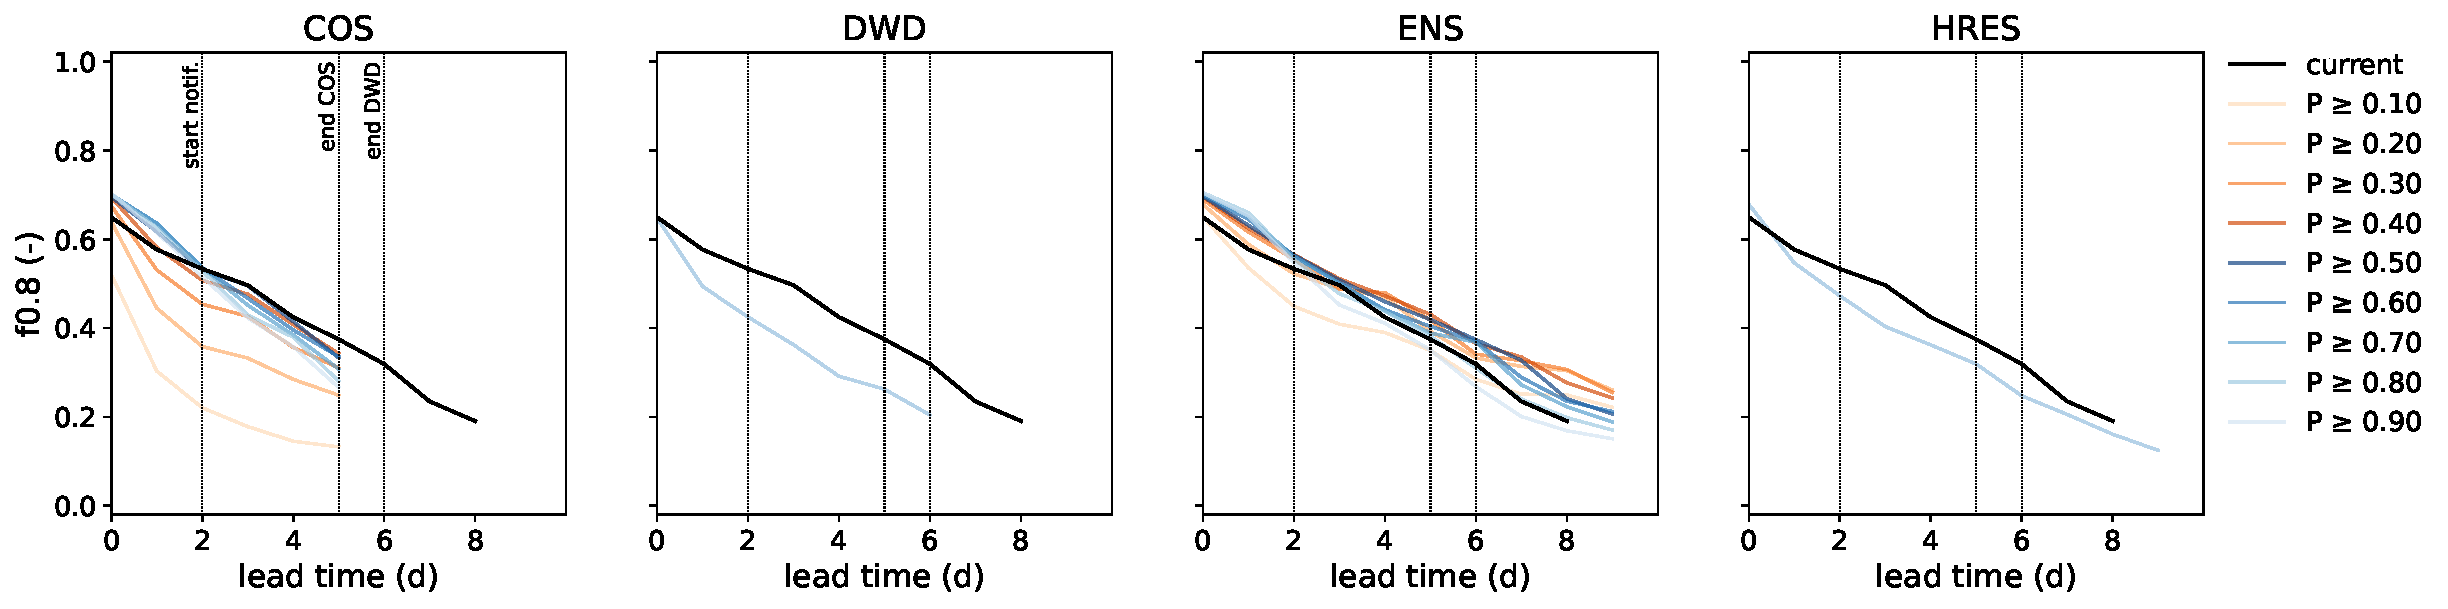
\includegraphics[width=1\textwidth]{figures/skill_probability_leadtime_1-1_NWP.pdf}
    \caption{Evolution of the notification skill with daily lead times and probability threshold for each NWP model in an scenario with no persistence. Each plot represents a different NWP. As a benchmark, the black, solid line represents the skill of the current operational criteria (1 deterministic + 1 probabilistic, 30\% probability and a persistence of 3 forecasts).}
    \label{fig:NWP_skill_leadtime}
\end{figure}

In line with Figure \ref{fig:BSS}, the probabilistic models are more skillful than the deterministic. Under some conditions, they even outperform the current notification criteria, which means that there is ground for improving the skill of EFAS. Deterministic models are as skillful as the current criteria only for the very first lead time.

As expected, notification skill degrades with lead time. This applies to all cases (deterministic, probabilistic and benchmark), but the rate of degradation is affected by the probability threshold. Low probability thresholds degrade sharply at short lead times, and high probability thresholds have a larger loss of skill at long lead times (see EUE over 7 days). 

There is a range of probability thresholds from approximately 40\% to 80\% with similar good skill. Within this range, larger thresholds perform slightly better at short lead times, and lower thresholds perform slightly better at mid-long lead times. Since we need to find out a single probability threshold for the notification criteria, the selection of the optimal criteria will focus on a lead time range from 2 days (the minimum formal notification lead time) to 5.5 days (the maximum lead time in COS). In this range we avoid the large uncertainty at long lead times and we focus on the lead times at which the majority of the formal notifications are issued.

So far, we have removed persistence from the exploration. To evaluate the effects of persistence in the notification skill we have produced the plot in Figure \ref{fig:NWP_skill_probability}, which shows the evolution of skill with the probability threshold and persistence for a fixed lead time range (2-5.5 days). The benchmark (current notification criteria) is now a single point corresponding the 30\% probability and persistence 3/3. As the probability threshold does not affect deterministic forecasts, the lines for the two deterministic models (DWD and EUD) are horizontal.

\begin{figure}
    \centering
    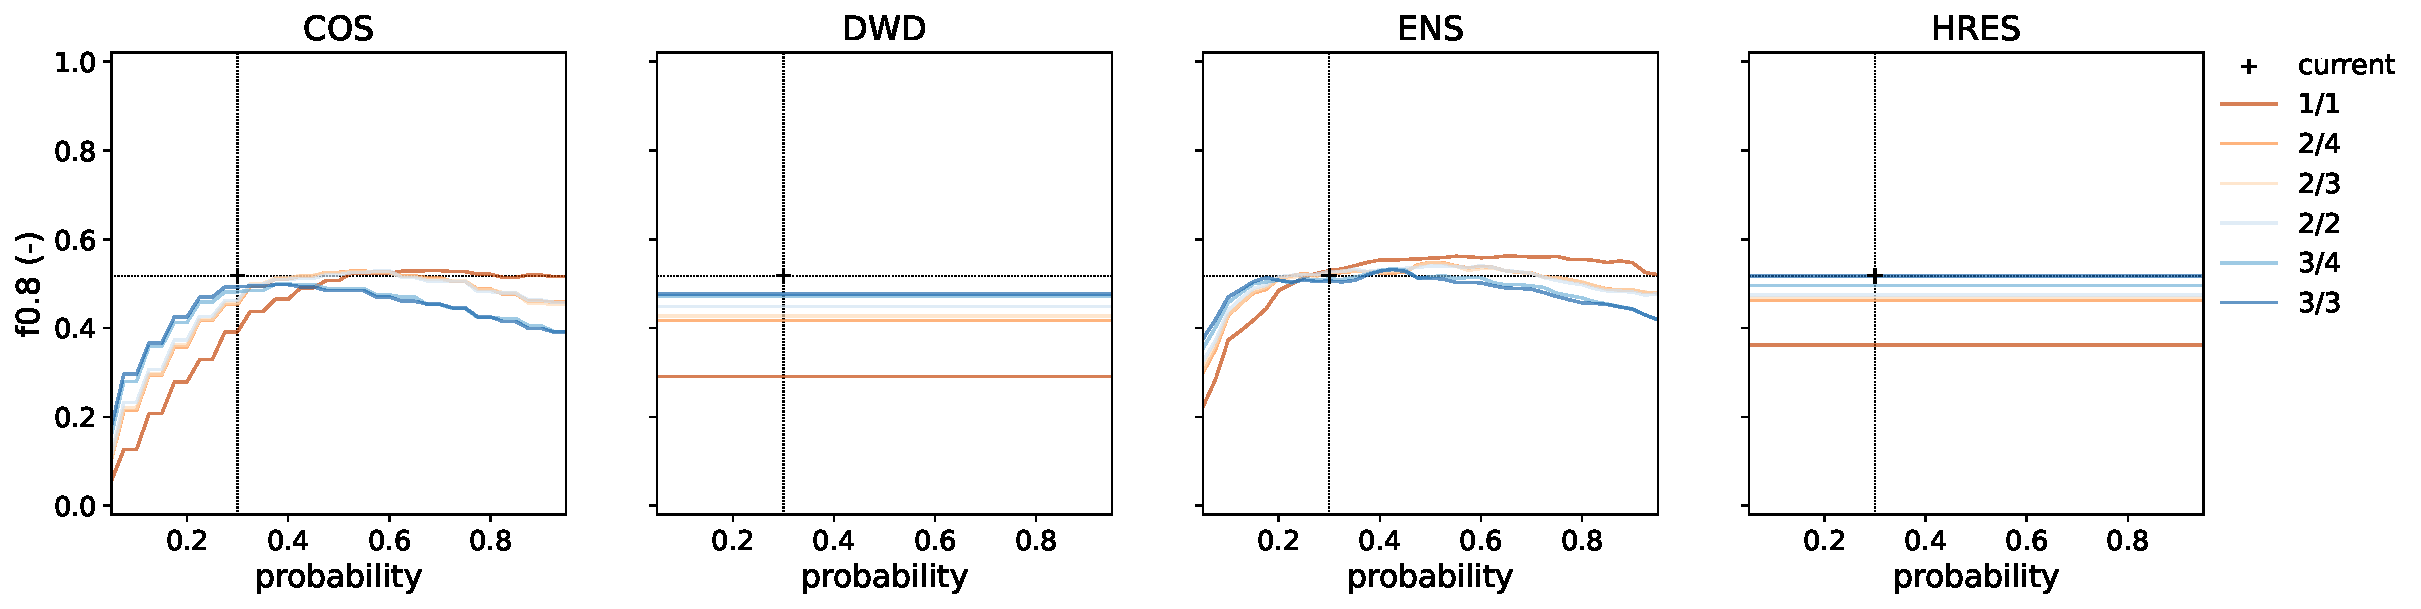
\includegraphics[width=1\textwidth]{figures/skill_persistence_probability_060h_NWP.pdf}
    \caption{Evolution of the notification skill with probability threshold and persistence  for each NWP model at a fixed lead time range (from 2 to 5.5 days). Each plot represents a different NWP model. As a benchmark, the black dot represents the current criteria (1 deterministic + 1 probabilistic, 30\% probability and a persistence of 3 forecasts).}
    \label{fig:NWP_skill_probability}
\end{figure}

Three out of four NWP models are able to replicate or improved the skill of the current notification criteria at some combinations of persistence and probability. Only DWD is less skillful than the benchmark.

The skill of the probabilistic models shows a trade-off between probability threshold and persistence. Both criteria play the same role, which is removing false positives (or uncertain events) by taking stricter values. Hence, increasing values of persistence require lower probability thresholds to optimize the skill. Nevertheless, the scenario of no persistence produces the highest notification skill. At this scenario, there is a wide range of probability thresholds (from 40/50\% to 90\%) that perform similarly good.

Persistence does make a larger difference in the deterministic models. Their skill improves dramatically as soon as some persistence is added in the criteria. For the most stringent persistence (3/3), the skill of the deterministic EUD is as good as that of the probabilistic EUE, and even better than COSMO-LEPS. However, as explained earlier, this is a sub-optimal set of criteria; it does not outperform the probabilistic models with no persistence.

With the knowledge gained in the previous exploration, we were in a better position to optimize the notification criteria and understand the results. Table 1 summarizes the results of the optimization of notification criteria for the individual NWP models. The results are organised by lead time ranges; for each range, the table presents the optimized criteria (probability and persistence) and the skill metrics (recall, precision and f0.8) for the available NWP models. As a benchmark, the first row in each lead time range shows the skill of the current operational criteria. The objective of the optimization is two-fold: first, to compare the optimal skill of the different NWPs, second, to set a baseline against which we can assess the added value of combining all NWPs.

\begin{table}
    \centering
    \caption{Summary of the optimization of the notification criteria for individual NWP and four lead time ranges. Skill metrics refer to the complete set of reporting points.  The initial row serves as a benchmark, indicating the skill of the current notification criteria. In each lead time range, bold figures highlight the peak value for a specific metric.}
    \footnotesize
    \begin{tabular}{cccccccc}
        \toprule
        lead time & model & probability & persistence & recall & precision & $\text{f}_{0.8}$ & rank \\
        \midrule
        \textless 2 d & 1D+1P & 0.300& 3/3 & 0.522 & \textbf{0.735} & 0.634 & 3 \\
         & COS & 0.875 & 1/1 & 0.673 & 0.718 & \textbf{0.700} & 1 \\
         & DWD & - & 2/2 & 0.585 & 0.583 & 0.583 & 5 \\
         & EUD & - & 2/2 & 0.580 & 0.671 & 0.632 & 4 \\
         & EUE & 0.800 & 1/1 & \textbf{0.681} & 0.711 & 0.699 & 2 \\
         \midrule
        2-5.5 d & 1D+1P & 0.300& 3/3 & 0.413 & 0.618 & 0.518 & 3 \\
         & COS & 0.725 & 1/1 & 0.387 & 0.687 & 0.518 & 2 \\
         & DWD & - & 3/3 & \textbf{0.420} & 0.522 & 0.477 & 5 \\
         & EUD & - & 3/3 & 0.416 & 0.612 & 0.517 & 4 \\
         & EUE & 0.650 & 1/1 & 0.416 & \textbf{0.725} & \textbf{0.562} & 1 \\
         \midrule
        5.5-7 d & 1D+1P & 0.300& 3/3 & 0.215 & \textbf{0.612} & 0.356 & 2 \\
         & DWD & - & 2/2 & \textbf{0.291} & 0.358 & 0.328 & 4 \\
         & EUD & - & 2/2 & 0.273 & 0.429 & 0.351 & 3 \\
         & EUE & 0.450 & 1/1 & 0.264 & 0.605 & \textbf{0.402} & 1 \\
         \midrule
        7-10 d & 1D+1P & 0.300& 3/3 & 0.120 & \textbf{0.625} & 0.237 & 3 \\
         & EUD & - & 2/2 & 0.244 & 0.336 & 0.293 & 2 \\
         & EUE & 0.175 & 2/2 & \textbf{0.287} & 0.396 & \textbf{0.345} & 1 \\
         \bottomrule
    \end{tabular}
    \label{tab:NWP_optimization}
\end{table}

When looking at the f-score, the current notification criteria (1D+1P) are outperformed at any lead time range by at least one NWP. If we focus in the lead time range from 2 to 5.5 days, the current criteria are able to notify 41\% of the events (recall) and 62\% of the notifications are correct (precision). The current criteria seem too strict, i.e., notifications are issued only with a high level of certainty. Whenever sent, they turn out to be mostly correct, but many events are missed. If we turn this values into skill (see Table 1), the current criteria  has an $f_{0.8}$ score of 0.518.

For the first lead time range, the best NWP is COS, with EUE showing almost equal skill. Both EUE and COS optimized a very high probability threshold and persistence was not required. The skill of the 2 deterministic NWP is distinctively lower, especially in the case of DWD. The 2 models optimized a persistence of 2/2. When comparing the skill of individual NWP with the current operational criteria, we find out that any of the 2 probabilistic models independently outperform the current criteria, and the deterministic EUD almost reaches the benchmark skill.

The picture does not change when looking at lead times from 2 to 5.5 days. The 2 probabilistic NWP have a higher skill than the deterministic ones and outperform the current operational criteria, but in this case EUE is the best NWP. Neither of the probabilistic models require persistence and the probability thresholds are lower than in the previous lead time range, but still higher than the 30\% value used currently. Again the deterministic models require a persistence of 3, and EUD almost equals the benchmark skill. Overall, there is a loss in skill of approximately 20\% compared with the first 2 days of forecast. 

For lead times from 5.5 to 7 days COS is not available any more. The only probabilistic model, EUE, outperforms the deterministic models and the benchmark. The probability threshold optimized for this lead time range is lower than in shorter lead times, but still larger than the current operational value. In general, there has been a loss in skill of approximately 30\% with respect to the previous lead time range (above 40\% compared with the first 2 days of forecast).

In the last 3 days of forecast only EUE and EUD are available. Both of the NWP models outperform the current criteria, but EUE is clearly more skillful than EUD. This long lead time range is the only one for which EUE required persistence (2/2), whereas the probability threshold is slightly lower than in the previous range.

Comment the Roebber diagram!!! Negatively biases, i.e., EFAS produces less notifications that the number of actual events.

\begin{figure}
    \centering
    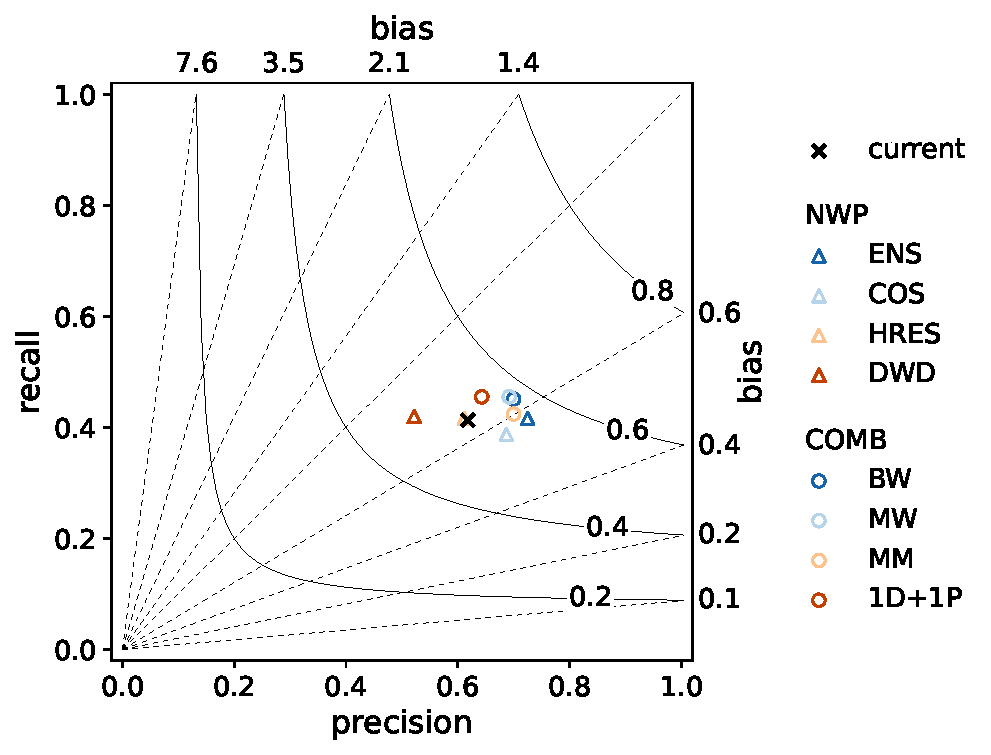
\includegraphics[width=0.5\linewidth]{figures/roebber_fscore_60h.pdf}
    \caption{Roebber diagram of the optimized criteria at the lead time range from 2 to 5.5 days. Triangles represent individual NWP and circles the 4 combination of NWP tested in this work. As a reference, the skill of the current notification criteria is been added as a black cross. The Roebber diagram shows in a single plot 4 skill metrics: precision and recall in the X and Y axis, bias is represented by the dashed lines, and the f0.8 score by the solid lines.} 
    \label{fig:roebber_NWP}
\end{figure}

\subsection{Combination of models}
\label{sec:results_COMB}

Three of the four combination methods compute total probability. To do so weights need to be assigned to every NWP. Figure \ref{fig:weights} shows the distribution of weights among NWP models for those three combination methods, and how the weights change with lead time.

\begin{figure}
    \centering
    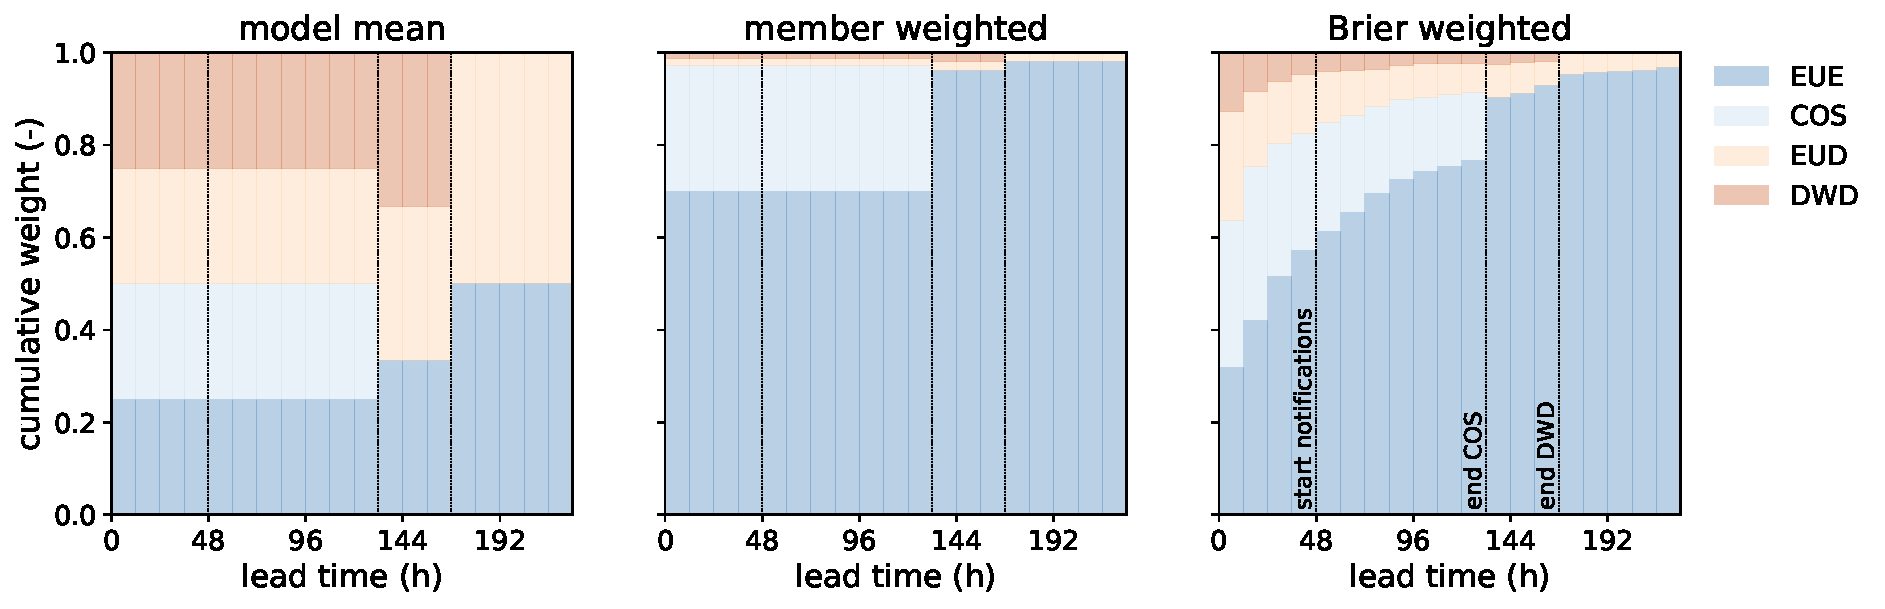
\includegraphics[width=1\textwidth]{figures/weights.pdf}
    \caption{Weights applied to compute the total probability out of the NWP models. Every plot represents a different approach. Colours represent the NWP (blue for probabilistic and orange for deterministic models).}
    \label{fig:weights}
\end{figure}

The model mean (MM) approach attributes equal weights to each model. The changes in the weights with lead time occur when the maximum lead time of a model is exceeded (5.5 days for COS and 7 days for DWD). This is the approach in which the deterministic models are given the same importance as the probabilistic models.

In the member weighted (MW) combination, every model run is assigned an equal weight. Therefore, EUE, which has a significant larger number of members, prevails over any other NWP. Even for the first 5 days, when all the models are available, EUE gets 70\% of the weight. Instead, the sum of the two deterministic models (EUD and DWD) has a maximum weight of 4\% from days 5.5 to 7. If we compare these weights to the current 30\% probability criterion, it means that in the case that EUE completely fails to predict an event, the 30\% total probability could never be achieved at lead times longer than 5.5 days, and only if all the other models were completely correct would the event be notified at lead times shorter than 5.5 days. In general, this approach relies heavily on the skill of EUE, which fortunately is the most skillful model (see Figure \ref{fig:BSS}).

In the Brier weighted (BW) combination, the Brier score values from section \ref{sec:NWP_prob_skill} were transformed to be used as weighing factors in the computation of the total probability. This transformation consisted of re-scaling the original values by inverse distance weighing, so that the sum of all weights is 1. The resulting weights vary with lead time, showing a transition from short to long lead times. At very short lead times the deterministic models are skillful, so they sum up to a third of the weight. As the lead time increases, the probabilistic models, especially EUE, take most of the weight. At lead times from 2 to 5.5 days, when most of the notifications are sent, the probabilistic models carry at least 80\% of the weight.

\subsubsection{Notification skill}
\label{sec:COMB_skill}

Figure \ref{fig:COMB_skill_leadtime} and Figure \ref{fig:COMB_skill_probability} replicate the analysis of the notification skill previously done for the individual NWP models, but this time for the combination methods. Figure \ref{fig:COMB_skill_leadtime} shows the evolution of the notification skill with lead time and probability threshold for a fixed persistence value (no persistence). Figure \ref{fig:COMB_skill_probability} presents, instead, the evolution with probability and persistence for a fixed lead time range (2-5.5 days). Together they portray an overall picture of the behaviour of skill in the four dimensions: combination method, lead time, probability threshold and persistence.

\begin{figure}
    \centering
    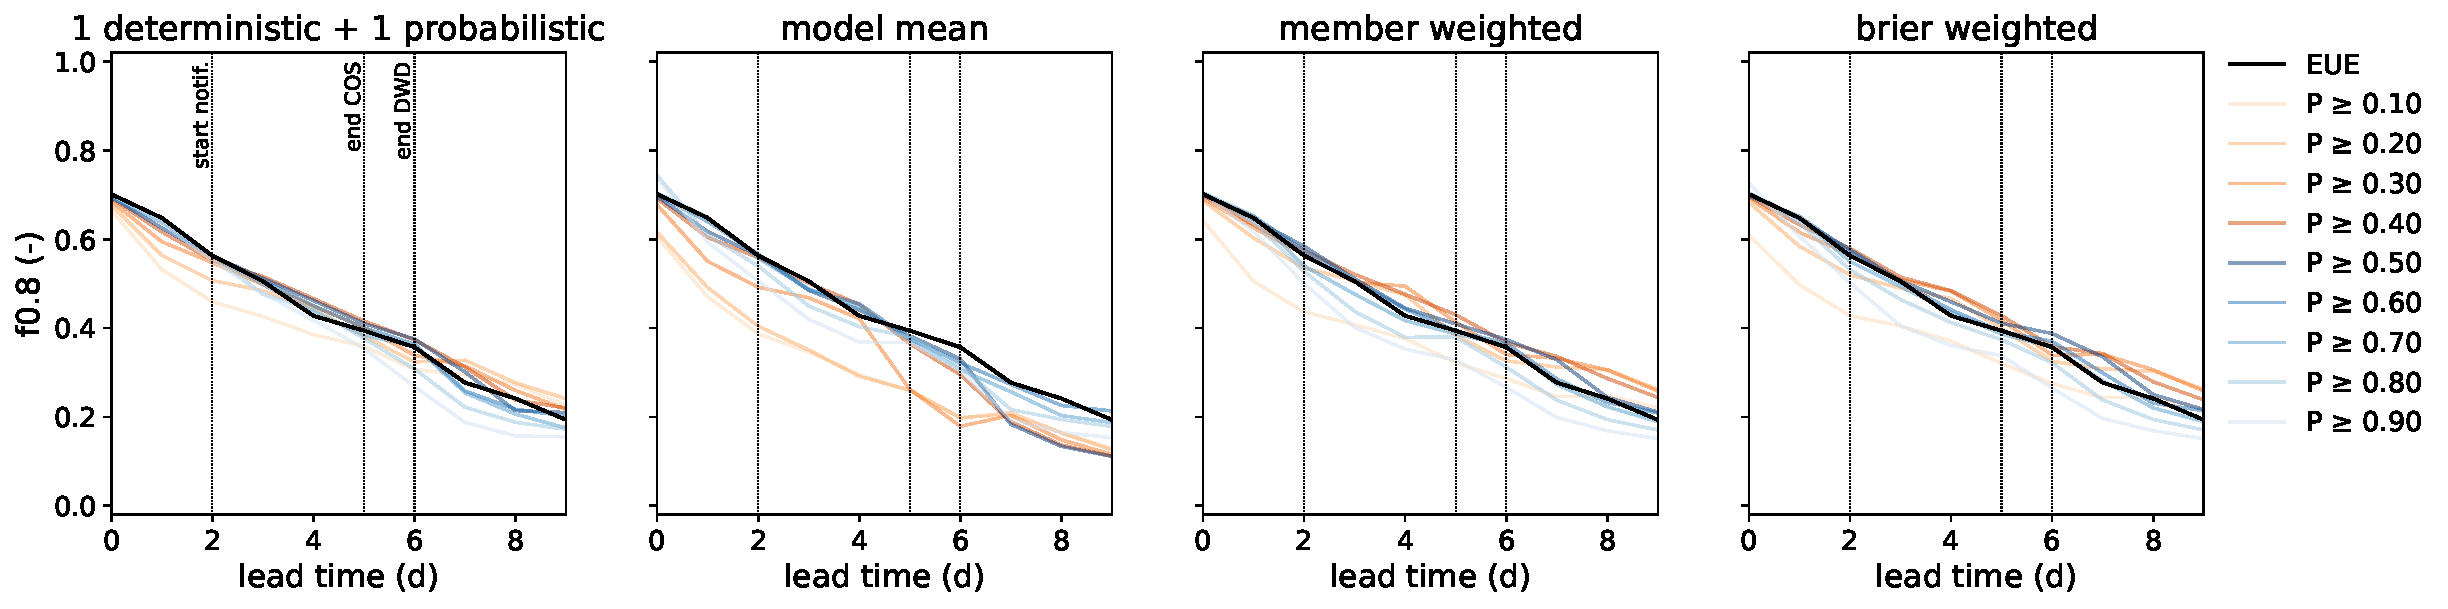
\includegraphics[width=1\textwidth]{figures/skill_probability_leadtime_1-1_COMB_vs_EUE.pdf}
    \caption{Evolution of the notification skill with daily lead times and probability threshold for each of the combination methods in an scenario with no persistence. Each plot represents a different combination of NWP. As a benchmark, the black, solid line represents the skill of EUE with optimized criteria (65\% probability and no persistence).}
    \label{fig:COMB_skill_leadtime}
\end{figure}

As EUE is the most skillful NWP, using it as a benchmark establishes  a tough competition. Three out four of combinations (1D+1P, MW, BW) are capable of adding value to the EUE benchmark, but only from lead time 4 onward. In any case, the improvement in skill is limited. The skill among combinations is fairly similar, but we can already notice that the member weighted  and Brier weighted  approaches slightly outperform the other two. Except for the model mean, larger probability thresholds perform better at short lead times and smaller thresholds at longer lead times. Despite that fact, there is equifinality in the optimum of the probability thresholds. This behaviour of the probability threshold was already seen in the individual NWP.

Regardless of the NWP or combination of NWP, the notification skill degrades notably with lead time. Even if at lead time 0 the skill is high (up to 0.74), the minimum lead time criterion limits the EFAS notification skill to values slightly lower than 0.6. The degradation continues and, from day 7 onward, the skill drops below 0.4, which may me an indicator for creating a new limitation on the maximum lead time at which notifications are issued.

\begin{figure}
    \centering
    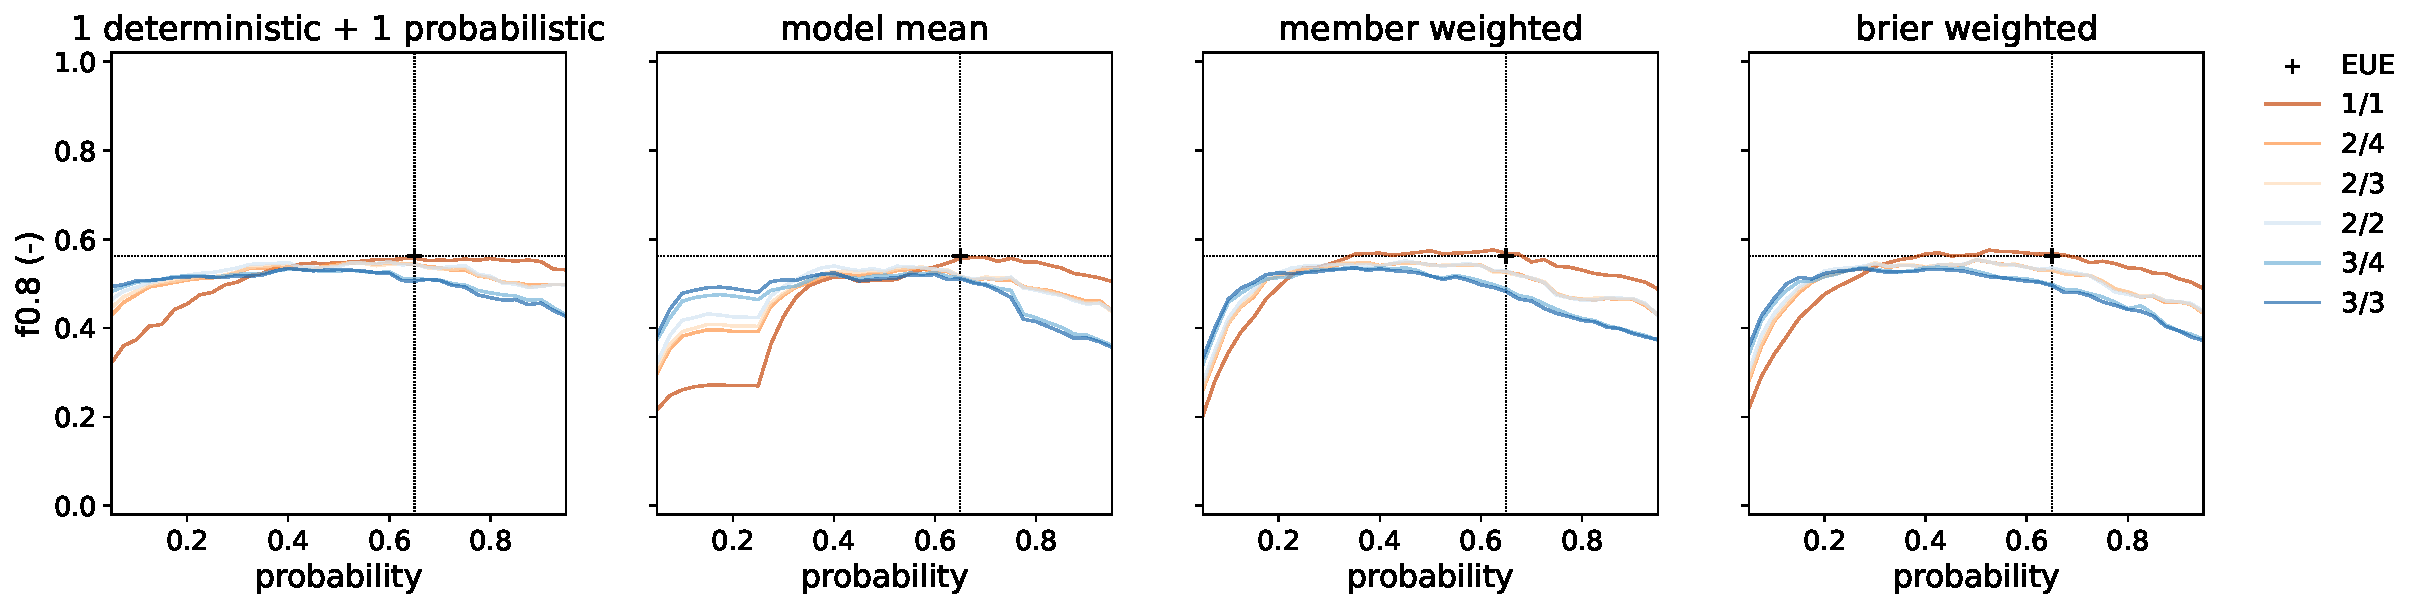
\includegraphics[width=1\textwidth]{figures/skill_persistence_probability_060h_COMB_vs_EUE.pdf}
    \caption{Evolution of the notification skill with probability threshold and persistence  for each combination of NWP at a fixed lead time range (from 2 to 5.5 days). Each plot represents a different NWP model. Each plot represents a different combination of NWP. As a benchmark, the black cross represents the skill of EUE with optimized criteria (65\% probability and no persistence).}
    \label{fig:COMB_skill_probability}
\end{figure}

Figure \ref{fig:COMB_skill_probability} proves that introducing the persistence criterion limits the maximum attainable skill. Across all four combinations, the highest skill is reached when no persistence is applied (1/1). In this scenario, all combinations exhibit similar maximum skill. Only member weighted (MW) and Brier weighted  (BW) marginally surpass the baseline (EUE). These two combinations show optimal skill within a range of probability thresholds spanning 40\% to 70\%. In both instances, the maximum skill is achieved at a probability threshold lower than that optimized for EUE.

The absence of sensitivity to probability in the current criteria (indicated by the dark blue line in the left-hand side pane) is noteworthy. Even at the lowest probability threshold, the f0.8 score remains at 0.5, unlike other approaches where there is a significant decline in performance as the probability threshold approaches very low values.

Table 2 summarizes the results of the optimization of the notification criteria for the combination methods in an identical way as Table 1 did for the NWP. The results are organised by lead time ranges; for each range, the table presents the optimized criteria (probability and persistence) and the skill metrics (recall, precision and f0.8) for the four methods. As a baseline, the first row in each lead time range shows the skill of EUE, which we established as the reference NWP in Table 1. The objective of the optimization is again two-fold: to compare the four combinations of NWP models, and to assess the added value of combining all NWPs instead of simply using the baseline. 

\begin{table}
    \centering
    \caption{Summary of the optimization of the notification criteria for the combination methods and four lead time ranges. Skill metrics refer to the complete set of reporting points. The initial row serves as a baseline, indicating the skill of EUE, the top-performing NWP. In each lead time range, bold figures highlight the peak value for a specific metric. }
    \begin{tabular}{cccccccc}
        \toprule
        lead time & method & probability & persistence & recall & precision & $f_{0.8}$ & rank \\
        \midrule
        \textless 2 d& EUE & 0.800 & 1/1 & \textbf{0.681} & 0.711 & 0.699 & 4 \\
         & 1D+1P & 0.925 & 1/1 & 0.662 & 0.717 & 0.694 & 5 \\
         & MM & 0.775 & 1/1 & 0.628 & \textbf{0.838} & \textbf{0.741} & 1 \\
         & MW & 0.750 & 1/1 & 0.673 & 0.718 & 0.700 & 3 \\
         & BW & 0.950 & 1/1 & 0.620 & 0.829 & 0.733 & 2 \\
         \midrule
        2-5.5 d & EUE & 0.650 & 1/1 & 0.416 & \textbf{0.725} & 0.562 & 3 \\
         & 1D+1P & 0.600 & 1/1 & \textbf{0.455} & 0.643 & 0.554 & 5 \\
         & MM & 0.700 & 1/1 & 0.424 & 0.700 & 0.559 & 4 \\
         & MW & 0.500 & 1/1 & \textbf{0.455} & 0.692 & 0.574 & 2 \\
         & BW & 0.525 & 1/1 & 0.451 & 0.700 & \textbf{0.576} & 1 \\
         \midrule
        5.5-7 d & EUE & 0.450 & 1/1 & 0.264 & \textbf{0.605} & \textbf{0.402} & 1 \\
         & 1D+1P & 0.425 & 1/1 & 0.262 & 0.599 & 0.399 & 4 \\
         & MM & 0.500 & 1/1 & \textbf{0.276} & 0.412 & 0.345 & 5 \\
         & MW & 0.425 & 1/1 & 0.271 & 0.579 & 0.401 & 2 \\
         & BW & 0.450 & 1/1 & 0.268 & 0.586 & 0.400 & 3 \\
         \midrule
        7-10 d & EUE & 0.175 & 2/2 & \textbf{0.287} & 0.396 & \textbf{0.345} & 1 \\
         & 1D+1P & 0.250 & 1/1 & 0.256 & 0.414 & 0.334 & 4 \\
         & MM & 0.225 & 2/2 & 0.252 & 0.334 & 0.296 & 5 \\
         & MW & 0.175 & 2/2 & 0.278 & 0.402 & 0.343 & 3 \\
         & BW & 0.300 & 1/1 & 0.255 & \textbf{0.445} & \textbf{0.345} & 1 \\
         \bottomrule
    \end{tabular}
    \label{tab:COMB_optimization}
\end{table}

In the shortest lead time range, two combinations clearly outperform the baseline (MM, BW). Between the two, MM exhibits the highest skill ($f_{0.8}=0.741$). This proficiency can be attributed to MM emphasis on deterministic models, which demonstrated notable skill at very short lead times (see Figure \ref{fig:weights}). As of the optimized criteria, none of the four methods required persistence, and probability thresholds fell within the top quartile. At this lead time range EFAS formal notifications are not issued, so the results above are only informative, but do not affect the selection of new criteria.

From day 2 to 5.5, BW and WW stand out as the top-performing combinations, showcasing comparable skill that surpass the baseline. Both approaches operate optimally without the need for persistence, with the probability threshold hovering around 50\% (refer to Figure \ref{fig:COMB_skill_probability} for a sense of the uncertainty in defining the probability threshold). Compared with the preceding lead time range, there is an evident decline in skill by approximately 20\%. This is the lead time range at which most of the notifications are issued, so the decision about the new notification criteria will be based on this results.

In the third lead time range, from 5.5 to 7 days, none of the combinations outperform the baseline, despite three of them (1D+1P, MW and BW) attaining very similar skill. None of these three methods necessitated the use of persistence, and the associated probability thresholds were slightly lower than those in the preceding lead time range (around 40\%). When compared with the prior lead time range, there is a decrease in skill of around 30\% (45\% when compared to the the first range).

In the longest lead time range, BW emerges as the best-performing combination, with a skill on par with the baseline. MW, while slightly less proficient, shows similar skill. However, their optimized criteria differ. MW requires a persistence of 2 out of 2 forecasts and a relatively low probability threshold (0.175) — precisely the same criteria optimized for the baseline. In contrast, BW does not require persistence, and its probability threshold (30\%) aligns with the decreasing trend observed in previous lead time ranges.

If we chose the BW combination with no persistence and probability threshold 52.5\% as the optimal, the distribution of hits, misses and false alarms would be that of Figure \ref{fig:maps_BW}. With this set of criteria EFAS would be able to predict 45\% of the events, and 70\% of the predictions would be correct. As a reminder, these figures were 41\% and 62\% for the current criteria.

\begin{figure}
    \centering
    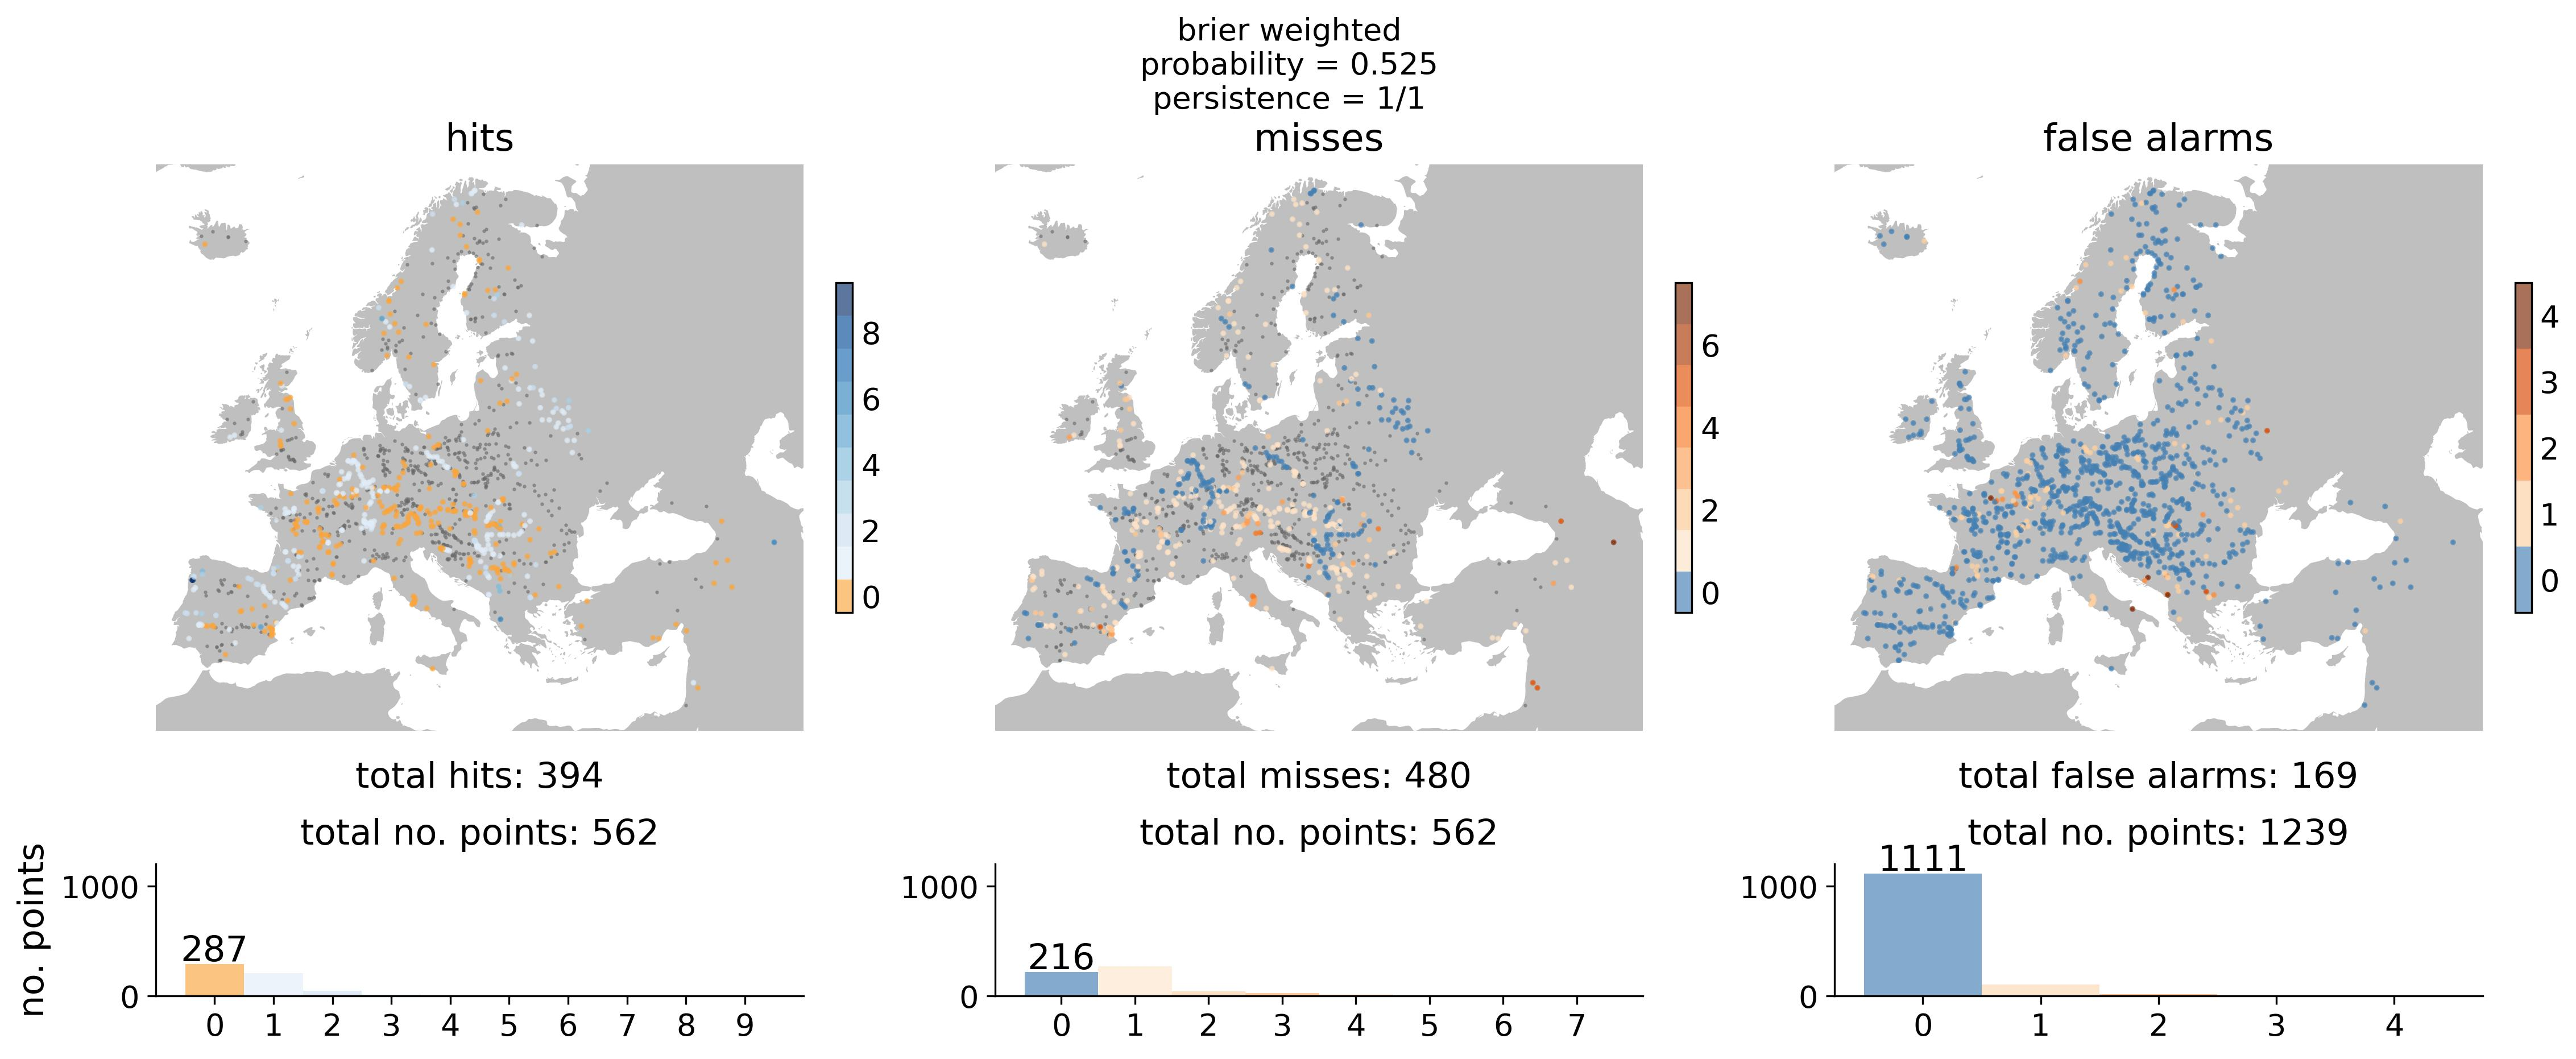
\includegraphics[width=1\textwidth]{figures/hits_maps_reporting_points_2000km2_1239points_brier_weighted_060h.jpg}
    \caption{Maps of hits, misses and false alarms for the highest-performing notification criteria. The colour scale changes depending on the variable; orange (darker orange) means worse values, whereas blue (darker blue) better values. In the case of hits and misses a mask has been applied to remove reporting points with no observed events (gray points), since none of these variables can be computed if there are no observations to be predicted or missed. The histograms at the bottom show the distributions of hits, misses and false alarms over the whole domain.}
    \label{fig:maps_BW}
\end{figure}

\subsection{Skill by catchment area}
\label{sec:skill_area}

The results of the previous sections refer to a set of reporting points with a catchment area of at least 2000 km², the current limit. To analyze whether this criterion could be relaxed, the plots in Figure \ref{fig:skill_area} describe the skill of the criteria, both current and optimized, according to the minimum catchment area. The solid lines represent the f0.8 score, and the dotted, horizontal lines the value of the probability threshold. A text shows the value of the optimized persistence (as a reminder, the current criterion is 3/3). This plot corresponds to lead times between 2 and 5.5 days.

\begin{figure}
    \centering
    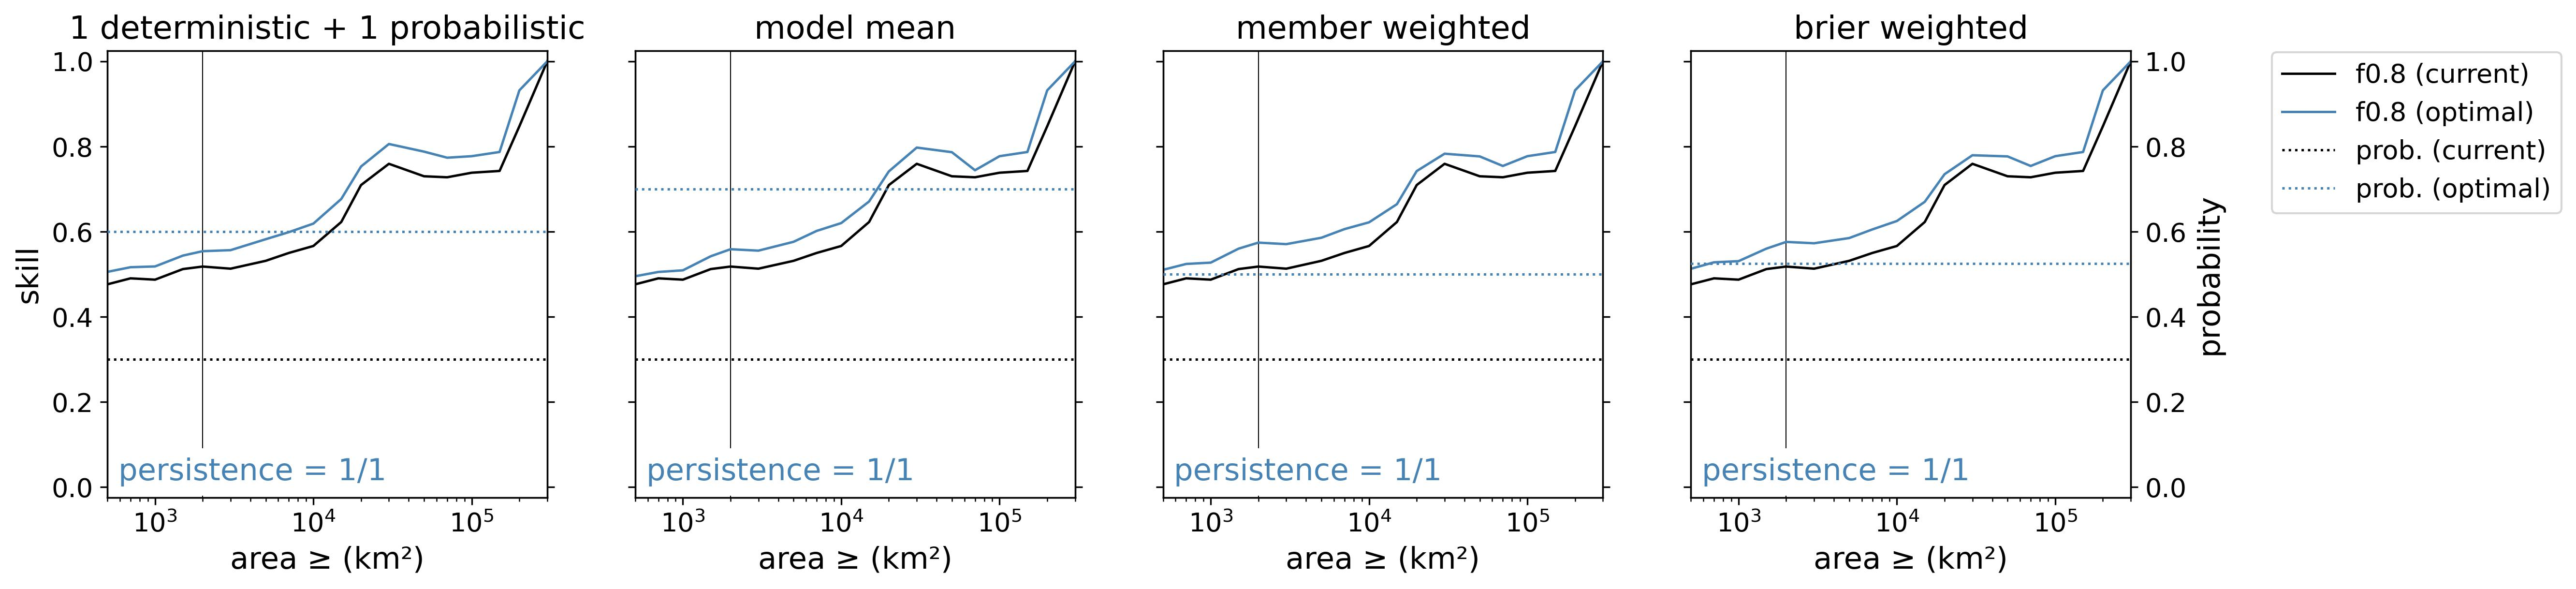
\includegraphics[width=1\textwidth]{figures/skill_vs_area_2000km2_1239points_060h.jpg}
    \caption{Evolution of skill with catchment area limit. Each plot represents a different combination of the NWP. The primary Y axis indicates skill, and the secondary Y axis indicates the probability threshold. The continuous lines are the target skill score (f0.8). The dotted lines are the probability thresholds. Black objects represent the current operational criteria and blue ones the criteria optimized for a fixed area threshold (represented by the vertical, solid, black line).}
    \label{fig:skill_area}
\end{figure}

The skill of the system improves with catchment area, as it was expected. Very large catchments have a f0.8 close to 1. However, the curves are not continuously increasing; in the areas ranging from 30,000 to 70,000 km² there is a loss of skill due to poor performance in the Guadiana, Seine, Loire, Rhone and Danube catchments. The vertical line at 2000 km² shows the gain in skill achieved with the optimization. This gain in skill seen at 2000 km² expands throughout all the catchment area values. When moving towards smaller catchments the loss in skill is minimal, which means that the catchment threshold could be reduced without compromising skill. For instance, the skill of the Brier weighted approach at 1000 km² (f0.8=0.531) is a bit higher than that of the current criteria at 2000 km² (f0.8=0.518).

In the previous analysis the probability threshold was fixed for any catchment area. But, what if we tune the probability threshold according to catchment area? Would it improved the skill of the system? The answer to this question is in Figure \ref{fig:skill_area_probability}. This figure is similar to Figure \ref{fig:skill_area}, but the comparison now is between the criteria optimized for the fixed area threshold of 2000 km² (blue) and for a varying area threshold (orange). We fixed the persistence value to that optimized previously and we only varied the probability threshold (dotted lines) for increasing area limits.

\begin{figure}
    \centering
    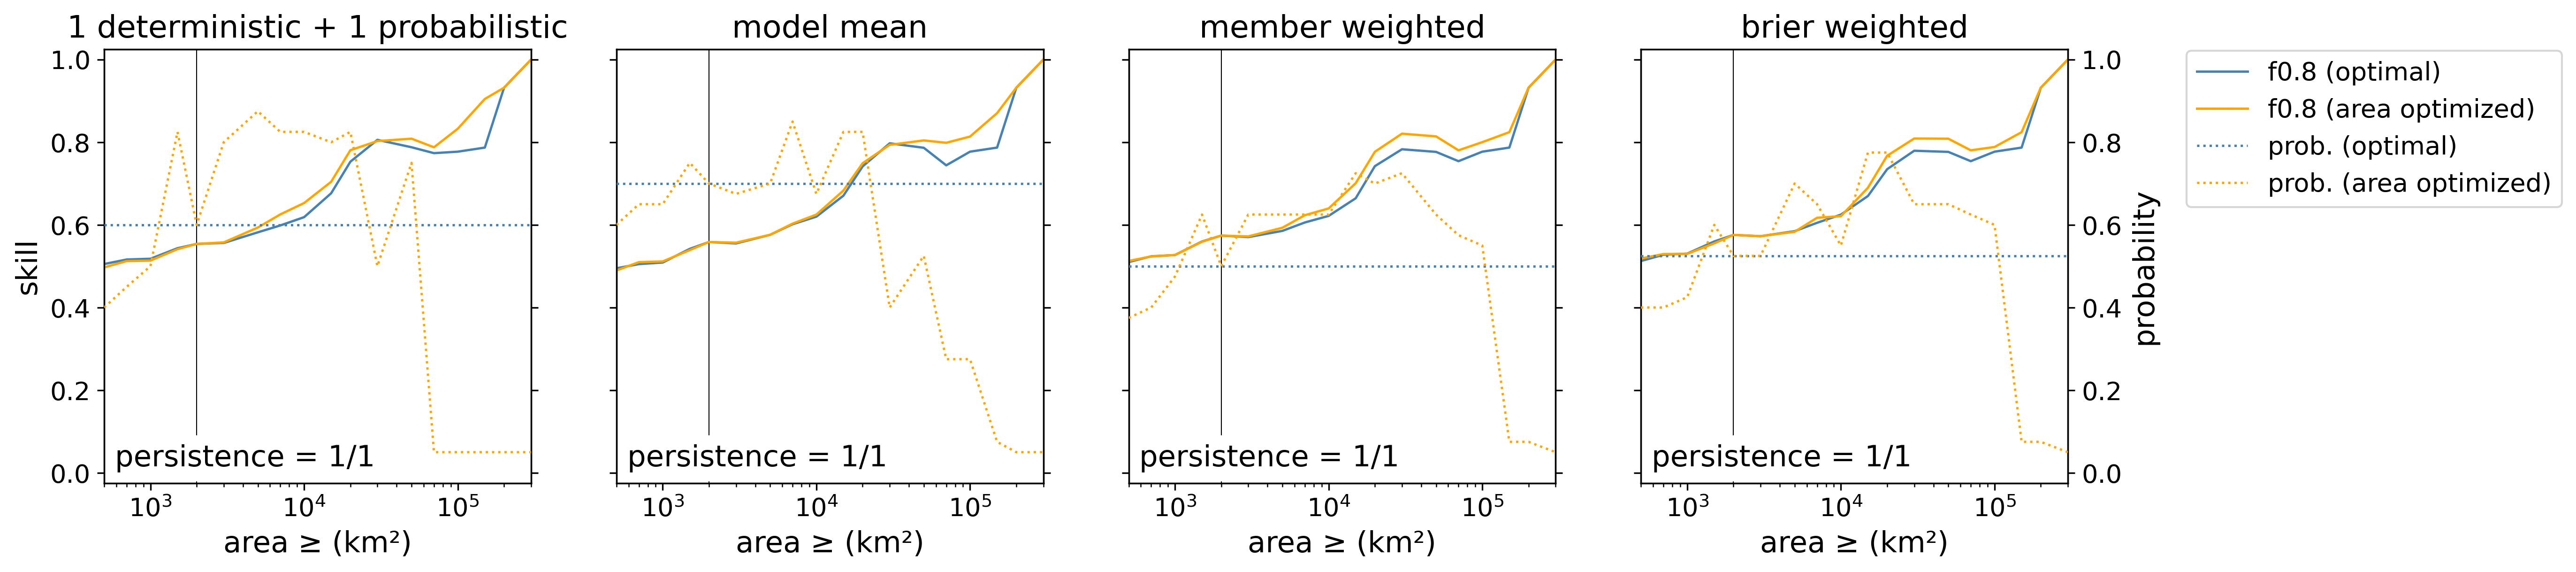
\includegraphics[width=1\textwidth]{figures/skill_vs_area_varying_probability_2000km2_1239points_060h.jpg}
    \caption{Evolution of skill with catchment area threshold. Each plot represents a different approach in which the meteorological forcing are combined. The primary Y axis indicates skill, and the secondary Y axis indicates the probability threshold. The continuous lines are the target skill score (f0.8). The dotted lines show the probability threshold. Blue objects are the results of the optimization with a fixed area threshold (represented by a vertical, solid, black line), and orange objects those for the optimization for every area threshold.}
    \label{fig:skill_area_probability}
\end{figure}

The skill measured as f0.8 is very similar for both optimizations. For areas lower than 2000 km² the skill is practically the same. For larger areas, the main improvement is at the range between 30,000 and 100,000 km², for which the fixed criteria shows a loss in skill. The biggest improvement is achieved in the 1 deterministic + 1 probabilistic and the  brier weighted approaches. The evolution of the probability threshold with catchment area is a bit erratic, probably due to the uncertainty in defining the optimal value (see Figure \ref{fig:COMB_skill_probability}), but a general trend can be guessed. The threshold takes lower values for catchment areas below the 2000 km² threshold, it peaks at a catchment area limit in the order of 100,000 km², and it drops to the minimum value of 5\% for very large catchments.

The main outcome of this experiment is that the global skill of the system does not improve significantly with a varying probability threshold. Therefore, for the sake of simplicity, a fixed probability threshold is advisable.

\section{Discussion}
\label{sec:discussion}

Three ideas can be extracted from the exploration of the notification skill in the individual NWP:
\begin{itemize}
    \item Probabilistic models, specifically ECMWF-ENS, are the most skillful and could outperform the current notification criteria under specific conditions. This idea is clearer in Figure \ref{fig:NWP_skill_probability}, which shows skill with no persistence.
    \item There is a range of equally good performing probability thresholds.
    \item The persistence criterion is very useful for the deterministic models, which are the least-performing, but hinders the skill of probabilistic models.
\end{itemize}

The conclusions of the optimization of criteria for the individual NWP:
\begin{itemize}
    \item Individual models outperform the current notification criteria. Even a deterministic model as EUD has similar skill.
    \item EUE will be the baseline for the combination methods, since it has proven to be the most skillful model.

\end{itemize}

The conclusions of the optimization of criteria for the combination of NWP:

\begin{itemize}
    \item ECMWF-ENS is a tough baseline, that was only clearly outperformed for the first 2 days lead time.
    \item Member weighted  and Brier weighted  are the two most promising approaches. When looking at the most interesting lead time range (48-132 h):
    \begin{itemize}
        \item Their skill is fairly the same.
        \item Their optimal criteria is similar: no persistence and a probability threshold around 50\%.
    \end{itemize}
\end{itemize}  

The decision about the most appropriate approach between MW and BW can not be based purely on skill metrics, but on other factors such as how easy it can be implemented operationally, how easy it is to be understood by the EFAS partners, or how it would be affected by removing or adding other meteorological models. BW seems to be the most logic approach as it grants higher importance to the most skillful models. It would also be the most robust approach in case of removing or adding NWP models. These two approaches perform equally good because they grant EUE (the model with highest skill and the largest number of members) most of the weight. If a more skillful model with fewer members would be added, BW would be able to extract that value more easily than MW. On the contrary, MW seems simpler to implement and would not require to run reforecasts whenever there is a new EFAS version or a new NWP model.

\section{Conclusions}
\label{sec:conclusions}

This study has analysed the skill of the notification criteria based on EFAS4 discharge simulations. The benchmark done with the current operational criteria shows that the system has an overall medium skill, with a tendency to underpredict events, i.e., to produce more missed events than false alarms.

An analysis of the individual meteorological models has shown that the two probabilistic models (COSMO-LEPS and ECMWF-ENS) individually outperform the current criteria, which uses four models. ECMWF-ENS is the most skillful model and will be used as a baseline for the optimization of the combination methods. The optimization of the notification criteria for the individual models NWP indicates that persistence is only a useful criteria for deterministic models, and that there is a certain degree of uncertainty in the definition of the optimal probability threshold for the probabilistic models (a wide range of probabilities perform equally good).

A second analysis compared the best NWP model against four different methods of combining the NWP models. From more simple to more complex, the model mean assigns the same value to all 4 NWP models, the member weighted method assigns equal value to every model run (probabilistic models prevail over deterministic), and the Brier weighted method uses the Brier score derived in the first analysis to weight the models according to their skill. The results prove that ECMWF-ENS is a baseline difficult to beat. Two approaches stand out as the most appropriate: member weighted  and Brier weighted . When looking at the most representative lead time range (60-132 h), they both outperform slightly the baseline, which means that they are able to add value from COSMO-LEPS, DWD or ECMWF-HRES to it. Both approaches optimized similar criteria: no persistence and a probability threshold around 50\%. The selection of one of these two approaches must be based on implementation issues, ability to add/remove meteorological forcing, and the interpretability on the part of EFAS partners.

Finally, we have analysed the possibility of relaxing the current criterion that establishes a minimum catchment area of 2,000 km². The results indicate that skill deteriorates with decreasing catchment area at a rather small rate. We have proven that with the optimized criteria we can achieve a similar performance at 1,000 km² as that of the current criteria at 2,000 km². We propose to reduce the limit at 1000 km² and, depending on the outcome of the flash flood skill assessment, further reduce it to 500 km² in the future.

Future work:

\begin{itemize}
\item In the future, when EFAS5 reforecast will be available, it will be interesting to redo the analysis for this version, especially regarding the question about reducing the area threshold.
\end{itemize}

\section{Data availability}

The reanalysis discharge data was downloaded from the \href{https://cds.climate.copernicus.eu}{Climate Data Store}. The forecast discharge data was extracted from the ECMWF Meteorological Archival and Retrieval System. The data set of reporting points was provided by HYDRO. All the scripts, pre-processed data and results of the analysis can be found in this \href{https://github.com/casadoj/EFAS_skill}{GitHub repository}.

%% The Appendices part is started with the command \appendix;
%% appendix sections are then done as normal sections
\appendix

\section{Sample Appendix Section}
\label{sec:sample:appendix}


%% If you have bibdatabase file and want bibtex to generate the
%% bibitems, please use
%%
 \bibliographystyle{elsarticle-num} 
 \bibliography{EFAS_skill}

%% else use the following coding to input the bibitems directly in the
%% TeX file.

% \begin{thebibliography}{00}

% %% \bibitem{label}
% %% Text of bibliographic item

% \bibitem{}

% \end{thebibliography}
\end{document}
\endinput
%%
%% End of file `elsarticle-template-num.tex'.
